% Some notes / rules:
% - Things marked \apw{} are APW's requests for Katie
% - Things marked \todo{} can be addressed by anyone

\documentclass[twocolumn]{aastex631}

% Packages
\usepackage{microtype}  % ALWAYS!
\usepackage{amsmath}
\usepackage{amsfonts}
\usepackage{amssymb}
\usepackage{multirow}

\definecolor{pink}{RGB}{232,132,161}
\newcommand{\kc}[1]{\textcolor{pink}{\textbf{#1}} }

\newcommand{\mlg}{\ensuremath{M_{\rm LG}}}
\newcommand{\mmto}{\ensuremath{M_{\rm M31}}}
\newcommand{\mmw}{\ensuremath{M_{\rm MW}}}
\newcommand{\vtan}{\ensuremath{v_\textrm{tan}}}
\newcommand{\vrad}{\ensuremath{v_\textrm{rad}}}
\newcommand{\mud}{\ensuremath{\mu_\delta}}
\newcommand{\mua}{\ensuremath{\mu_\alpha^*}}
\newcommand{\bov}{\ensuremath{\boldsymbol{v}}}
\newcommand{\boldx}{\ensuremath{\boldsymbol{x}}}
\newcommand{\vtrav}{\ensuremath{\bov_{\rm travel}}}
\newcommand{\xtrav}{\ensuremath{\boldx_{\rm travel}}}
\newcommand{\pos}[2]{\ensuremath{\boldx_{\rm #1 \to #2}}}
\newcommand{\vel}[2]{\ensuremath{\bov_{\rm #1 \to #2}}}
\newcommand{\mwbary}{\ensuremath{\textrm{MW}_\textrm{bary}}}
\newcommand{\mwouter}{\ensuremath{\textrm{MW}_\textrm{halo}}}
\newcommand{\mwdisk}{\ensuremath{\textrm{MW}_\textrm{disk}}}
\newcommand{\reflabel}[1]{\ensuremath{^{\mbox{\scriptsize{#1}}}}}

% Style tweaks
% \renewcommand{\twocolumngrid}{\onecolumngrid}
% \setlength{\parindent}{1.1\baselineskip}
% \sloppy\sloppypar\raggedbottom\frenchspacing

%%%%%%%%%%%%%%%%%%%%%%%%%%%%%%%%%%%%%%%%%%%%%%%%%%%%%%%%%%%%%%%%%%%%%%%%%%%%%%%%
\shorttitle{Updated Local Group Mass from Timing Argument}
\shortauthors{Chamberlain et al.}

%%%%%%%%%%%%%%%%%%%%%%%%%%%%%%%%%%%%%%%%%%%%%%%%%%%%%%%%%%%%%%%%%%%%%%%%%%%%%%%%
\graphicspath{{./}{figures/}}
% Missions
\newcommand{\project}[1]{\textsl{#1}}

% Packages / projects / programming
\newcommand{\package}[1]{\textsl{#1}}
\newcommand{\acronym}[1]{{\small{#1}}}
\newcommand{\github}{\package{GitHub}}
\newcommand{\python}{\package{Python}}
\newcommand{\astropy}{\package{Astropy}}

% Stats / probability
\newcommand{\given}{\,|\,}
\newcommand{\norm}{\mathcal{N}}
\newcommand{\pdf}{\textsl{pdf}}

% Maths
\newcommand{\dd}{\mathrm{d}}
\newcommand{\transpose}[1]{{#1}^{\mathsf{T}}}
\newcommand{\inverse}[1]{{#1}^{-1}}
\newcommand{\argmin}{\operatornamewithlimits{argmin}}
\newcommand{\mean}[1]{\left< #1 \right>}

% Non-scalar variables
\renewcommand{\vec}[1]{\ensuremath{\bs{#1}}}
\newcommand{\mat}[1]{\ensuremath{\mathbf{#1}}}

% Unit shortcuts
\newcommand{\Msun}{\ensuremath{\mathrm{M}_\odot}}
\newcommand{\Mjup}{\ensuremath{\mathrm{M}_{\mathrm{J}}}}
\newcommand{\kms}{\ensuremath{\mathrm{km}~\mathrm{s}^{-1}}}
\newcommand{\pc}{\ensuremath{\mathrm{pc}}}
\newcommand{\kpc}{\ensuremath{\mathrm{kpc}}}
\newcommand{\Mpc}{\ensuremath{\mathrm{Mpc}}}
\newcommand{\kmskpc}{\ensuremath{\mathrm{km}~\mathrm{s}^{-1}~\mathrm{kpc}^{-1}}}
\newcommand{\dayd}{\ensuremath{\mathrm{d}}}
\newcommand{\yr}{\ensuremath{\mathrm{yr}}}
\newcommand{\Kel}{\ensuremath{\mathrm{K}}}

% Misc.
\newcommand{\bs}[1]{\boldsymbol{#1}}

% Astronomy
\newcommand{\DM}{{\rm DM}}
\newcommand{\feh}{\ensuremath{{[{\rm Fe}/{\rm H}]}}}
\newcommand{\df}{\acronym{DF}}

% TO DO
\newcommand{\todo}[1]{{\color{red} TODO: #1}}
\newcommand{\apw]}[1]{{\color{green} APW says: #1}}

% Projects
\newcommand{\gaia}{\textsl{Gaia}}
\newcommand{\gaiadr}{\textsl{Gaia}~\acronym{EDR3}}


% Affiliations
\newcommand{\affuofa}{University of Arizona, 933 N. Cherry Ave,
    Tucson, AZ 85721, USA}
\newcommand{\affcca}{Center for Computational Astrophysics, Flatiron Institute,
    Simons Foundation, 162 Fifth Avenue, New York, NY 10010, USA}
\newcommand{\affedinb}{Institute for Astronomy, University of Edinburgh,
    Royal Observatory, Blackford Hill, Edinburgh EH9 3HJ, UK}
\newcommand{\affparis}{Institut d'Astrophysique de Paris,
    98 Bis Blvd Arago 75014 Paris, France}

%% This is the end of the preamble.  Indicate the beginning of the
%% manuscript itself with \begin{document}.

\begin{document}

\title{
  Implications of the travel velocity of the Milky Way on Local Group mass\\
  estimates from the Timing Argument
}

\author[0000-0001-8765-8670]{Katie~Chamberlain}
\affiliation{\affuofa}
\affiliation{\affcca}

\author[0000-0003-0872-7098]{Adrian~M.~Price-Whelan}
\affiliation{\affcca}

% TODO: Alphabetical ok?
\author[0000-0003-0715-2173]{Gurtina Besla}
\affiliation{\affuofa}

\author[0000-0002-6993-0826]{Emily C. Cunningham}
\affiliation{\affcca}

\author[0000-0001-7107-1744]{Nicol\'{a}s Garavito-Camargo}
\affiliation{\affcca}

\author{Jorge Pe\~{n}arrubia}
\affiliation{\affedinb}

\author[0000-0003-1517-3935 ]{Michael Petersen}
\affiliation{\affparis}

% TODO: Any other authors??

\begin{abstract}
    % \textbf{Context}
    The total mass of the Local Group (LG) is a fundamental quantity that
    enables interpretation of the orbits of its constituent galaxies and is
    needed to place the LG in a cosmological context.
    One of the few methods that enables inferring the total mass directly is the
    ``Timing Argument,'' which models the relative orbit of the Milky Way (MW)
    and M31.
    However, the MW is not in equilibrium with its dark matter halo, a byproduct
    of its merger history and the recent pericentric passage of the LMC.
    Recent studies of tracers in the MW stellar halo have found that
    the MW disk is moving with a lower bound “travel velocity” of $32\pm4$
    \kms\ with respect to its outer halo \citep{Petersen2021}, thus biasing past
    Timing Argument measurements that do not account for this motion.
    % \textbf{Aims}
    % \textbf{Methods}
    Here, we measure the total LG mass using a Timing Argument model that
    incorporates this measured ``travel velocity'' of the MW disk using several
    different compilations of recent kinematic measurements of M31.
    % \textbf{Results}
    We generally find lower LG masses than past Timing Argument results and
    measure a total mass of $4.5^{+0.8}_{-0.6}\times 10^{12}~\Msun$
    that is consistent between datasets.
    Measurements of the travel velocity with more distant tracers could yield
    even larger values, which would further decrease the inferred LG mass.
    Additionally, we find that future data releases from \emph{Gaia} will lead
    to more precise measurements
    of M31's proper motion that will improve the precision of Timing Argument
    mass constraints by a factor of $\sim2$.
    % \textbf{Conclusions}
    As a result, the newly measured travel velocity directly implies a lower LG
    mass than from a system with a static MW halo, and must be considered in
    future dynamical studies of the Local Volume.
\end{abstract}

\section{Introduction}
\label{sec:intro}
% \textbf{Importance of local group mass and measuring it}
% \todo{Review references - any obvious missing?}
The total mass of the Local Group is an important quantity in many local
cosmological and Milky Way (MW) applications.
For example, it is used to identify analogous halos in cosmological simulations
and thus allows comparing host galaxy and satellite galaxy number counts and
properties \citep[e.g.,][]{Patel2017a, Marinacci:2017, Dooley2017, Besla2018,
Patel2018, Garrison-Kimmel:2019a, Garrison-Kimmel:2019b, Sawala2022}.
It is also used to turn the kinematics of Local Group
galaxies into orbital histories \citep[e.g.,][]{Peebles:2017}, which is used to
interpret their gas content \citep[e.g.,][]{Fillingham:2018,Putman:2021} and
star formation histories \citep[e.g.,][]{Tolstoy:2009}.
However, as most of the mass in the Local Group is in dark matter distributed
over megaparsec scales, it is difficult to directly measure its total mass.

Given its utility in studies of the local universe, several methods have been
used to dynamically infer the mass of the Local Group.
Many of these techniques determine the individual masses of the MW and M31
independently \citep[e.g.][]{Watkins2010, Diaz2014, Patel2018, Eadie:2019,
Fritz:2020, Deason:2021, Wang:2022}, often via the dynamics of their satellites
and stellar streams, then combine them to get an estimate of the total LG mass.
However, these methods generally only measure the enclosed mass of the MW or M31
within some internal radius (i.e. much smaller than LG scales) and then
extrapolate, leading to mass-profile-dependent estimates of the total LG mass.
Other techniques aim to more directly measure the mass of the Local Group en
masse, for example looking for Local Group analogs in cosmological simulations
based on stellar mass and kinematic criteria \citep[e.g.,][]{Zhai2020}, or by
studying the kinematics of Local Volume galaxies
\citep[e.g.,][]{Penarrubia2014}.
One of the earliest methods utilized in this vein is the ``Timing Argument,''
which uses the fact that the local group galaxies (most often the MW and M31)
are bound and approaching pericenter in their relative orbit, but must have been
close enough over cosmic time to not be pulled apart by the Hubble flow. We
summarize the relevant details of the Timing Argument method in
Section~\ref{sec:timingarg}

The Timing Argument (using the MW and M31) uses the observed kinematics of M31
to model the relative orbit of the two galaxies as a Keplerian orbit.
Assuming Keplerian dynamics enables dynamically measuring the total mass of the
MW and M31 with analytic expressions for all relevant kinematic quantities
because of the simplicity of the two-body equations of motion.
The inferred mass from the Timing Argument is thus very sensitive to the
observationally-measured kinematics of the M31 center.

% the assembly of the Local Group is complicated and has been accounted for in
% The assembly history of the MW and M31 has an impact on the dynamics of the
% pair, as interactions and mergers with massive satellites lead to a
% non-equilibrium system.
% In particular, the Large Magellanic Cloud (LMC) is
% very massive ($\sim1/10$ of the total halo mass of the MW) and has
% likely recently made
% its first close pericentric passage around the MW \citep[see e.g.,][]{Besla2007,Patel2017a}. %\citep{}
Recent studies of the dynamics of the MW and its satellites have
revealed that the infall of the Magellanic Clouds (MCs) is likely causing
significant distortions to the dark matter and stellar distribution in the MW
halo \citep{Laporte:2018a, Laporte:2018b, Garavito-Camargo:2019, Conroy:2021,
Erkal:2021}, thus impacting the interpretation of observations of the M31
position and velocity relative to the MW center of mass.
Timing Argument studies that do not account for these perturbations are thus
likely only biased estimates of the LG mass.
\citet{Penarrubia2016} studied the impact of the presence of the LMC on the
total mass of the LG via the Timing Argument by explicitly modeling the masses
of the MW, LMC, and M31 as a dynamical system.
% as a function of the ratio between the LMC and MW masses.

In addition, numerous studies of the interaction between the MW and LMC (using
simulated analogs) have quantified the expected LMC-induced reflex motion of the
MW disk and inner halo, which are likely being accelerated away from the center
of mass reference frame of a static MW halo \citep{Gomez2015, Cunningham:2020,
Petersen:2020, Garavito-Camargo2021b}.
Recent Timing Argument work by \cite{Benisty2022} modelled the orbital history
of M31 and the MW with and without a mass model of the LMC to estimate the
contribution of the LMC-induced reflex motion of the MW to the measured
tangential and radial velocities of M31, then applied these corrections to their
model to remove the impact of the LMC in their analysis.
In fact, other satellite mergers such as the ongoing merger with the Sagittarius
dwarf galaxy, as well as the past merger with the progenitor of the
Gaia--Enceladus--Sausage, have likely also imparted their own reflex motion to
the inner MW halo.
Previous Timing Argument studies have therefore only accounted for the impact of
an LMC-induced reflex motion on the orbital histories of the other galaxies in
the LG.
% We have not simulated the cumulative effect of all previous MW mergers on the reflex motion of the disk, and so accounting for this through modelling is basically impossible.

However, recently the instantaneous velocity offset of the inner MW with respect
to the outer halo was directly measured using tracer stars in the stellar halo
of the MW (the ``travel velocity''; \citealt{Petersen2021}).
The measured travel velocity can thus be used in Timing Argument studies in
place of orbital modelling to account for the expected perturbations of the
inner MW halo without having to make assumptions about the mass or dynamical
history of the LMC or other satellites.

In this Article, we use the measured travel velocity of the inner Milky Way to
empirically infer the mass of the Local Group, thus accounting for observational
misinterpretations in a model-independent way for the first time.
We also explore a combination of recent measurements of the distance and proper
motions of M31 to infer the effect of the travel velocity in a
dataset-independent way.
As a result, we find that the travel velocity significantly impacts the inferred
mass of the LG in Timing Argument studies, and thus must be accounted for in
further dynamical studies of the Local Volume.


\section{Methods and Data}

%%%%%%%%%%%%%%%%%%%%%%%%%%%%%%%%%%%%
\subsection{Dynamical Model: The Timing Argument}
\label{sec:timingarg}
%%%%%%%%%%%%%%%%%%%%%%%%%%%%%%%%%%%%

Following past work that utilizes the ``Timing Argument,'' we assume that the
orbital trajectories of the MW and M31 --- the Local Group system --- over
cosmic history are well-described by Keplerian orbits \citep[e.g.,][]{Kahn1959,
Lynden-Bell:1981, Kroeker1991, LiWhite2008, vdm2012, Penarrubia2016}.
By assuming that M31 and the MW are gravitationally bound and were last at
closest approach in the early universe (i.e. the two galaxies have not yet
strongly interacted), we can then use the present-day kinematics of M31 relative
to the Milky Way to estimate the total mass of the Local Group (i.e. using the
Timing Argument).

% \textbf{The dynamics of the M31-MW system can be approximated by simple Keplerian orbits.}
In this work, we largely follow the methodology and notation defined in
\citet{Penarrubia2016}.
Briefly recapping the Timing Argument method, we assume that the dynamics of the
MW and M31 pair is dominated by the local gravitational potential of the Local Group
(LG) and therefore the Hubble flow can be neglected for computing the relative
orbits of the galaxies \citep[see, e.g.,][]{Penarrubia2014}.
Since we observe the relative position and motion between M31 and the MW, we
reduce the dynamics of the galaxies in the LG system to a single Keplerian orbit
that specifies the relative orbit between the galaxies and is completely
determined by four model parameters: the total mass of the Local Group \mlg, the
semi-major axis $a$, the eccentricity $e$, and the present value of the
eccentric anomaly $\eta$.

In terms of these four model parameters, the closed-form equations for relevant
two-body quantities that are closer to observables, like the separation between
the masses $r$, the elapsed time since last pericenter $t$, and the radial and
tangential velocity components \vrad\ and \vtan, are given by:
\begin{align}
  r &= a \, (1-e\,\cos\eta) \label{eq:r} \\
  t &= \left( \frac{a^3}{GM} \right)^{1/2}(\eta-e\,\sin\eta) \label{eq:t} \\
  \vrad &= \left( \frac{GM}{a} \right)^{1/2} \frac{e\,\sin\eta}{1-e\,\cos\eta} \label{eq:vrad} \\
  \vtan &= \left( \frac{GM}{a} \right)^{1/2} \frac{\sqrt{1-e^2}}{1-e\,\cos\eta} \label{eq:vtan} \quad .
\end{align}
In the expressions above, $r$ is the separation between the centers of the MW
and M31 halos, the time since last pericenter, $t$, is the age of the Universe,
and the velocity components, $(\vrad, \vtan)$, express the radial and tangential
velocity components of M31 relative to the center of the MW halo.

In a simpler universe where the MW and M31 are point masses and there are no
other massive bodies in the LG system, we could transform the observed
heliocentric sky position, distance, and velocity of M31 to a MW Galactocentric
reference frame and combine these with an estimate of the Hubble time to obtain
the four ``observables'' $(r, t, \vrad, \vtan)$:
These observables would be enough to infer the four model parameters $(\mlg, a,
e, \eta)$ using Equations~\ref{eq:r}--\ref{eq:vtan}.

To describe this ``classical'' Timing Argument approach in more detail and set
the stage for extending it, we adopt the notation of \citet{Penarrubia2016} in
which $\vel{A}{B}$ represents the velocity vector of A as measured in
the reference frame of B and $\pos{A}{B}$ represents the position vector of A as
measured from B.
With this notation, $\vel{A}{B} = -\vel{B}{A}$ and $\vel{A}{C} = \vel{A}{B} +
\vel{B}{C}$.

In the classical Timing Argument, the MW disk and M31 are assumed to occupy the
center of the potential well of their dark matter halos and have zero velocity
with respect to the halos.
We refer to this reference frame in the MW dark matter halo
as `\mwouter'.
Thus, the position and velocity of M31 with respect to the MW can be
represented by $\pos{M31}{\mwouter}$ and $\vel{M31}{\mwouter}$, which are
assumed to be equivalent to the position and velocity of M31 with respect to the
center of the MW disk.
Then, the \textit{observed} position and velocity of M31, measured in a heliocentric
reference frame, are given by
\begin{align}
  \pos{M31}{\odot} &= \pos{M31}{\mwouter} + \pos{\mwouter}{\odot} \label{eq:xoffset1}\\
  \vel{M31}{\odot} &= \vel{M31}{\mwouter} + \vel{\mwouter}{\odot} \label{eq:voffset1}\quad .
\end{align}
Here $\left|\pos{M31}{\mwouter}\right| = r$ as determined from
Equation~\ref{eq:r}, $\vel{M31}{\mwouter}$ is determined completely by the
Keplerian model parameters (through \vrad\ and \vtan), and the position and
velocity of the center of the MW halo as measured from the sun are
$\pos{\mwouter}{\odot}$ and $\vel{\mwouter}{\odot}$.

However, the true dynamics of the MW--M31 system are not so simple.
Perturbations introduced by interactions and mergers between the MW and its
satellite galaxies, such as the merger of the Sagittarius dwarf galaxy or the
recent pericentric passage of the LMC, break the assumption that the MW disk
is stationary in the center of its dark matter halo.
In fact, these interactions will introduce an additional reflex motion component
in observations from the MW disk compared to the \mwouter\ reference frame.
The LMC's impact on the dynamics of the MW disk and inner halo have been studied
in detail by~\cite[e.g.,][]{Gomez2015, Garavito-Camargo:2019, Petersen:2020,
Garavito-Camargo2021b}.
These works imply that we must include additional terms in
Equations~\ref{eq:xoffset1} and \ref{eq:voffset1} to account for the travel
velocity of the MW disk with respect to the center of the halo in its
unperturbed state.
Thus, the observed position and velocity vectors of M31 from the solar reference
frame become
\begin{align}
  \pos{M31}{\odot} &= \pos{M31}{\mwouter} + \pos{\mwouter}{\mwdisk}+\pos{\mwdisk}{\odot} \label{eq:xm31-solar}\\
  \vel{M31}{\odot} &= \vel{M31}{\mwouter} + \vel{\mwouter}{\mwdisk}+\vel{\mwdisk}{\odot}\label{eq:vm31-solar}
\end{align}
where ``\mwouter'' refers to a reference frame centered at and moving with the
center of mass of the outer MW halo, ``\mwdisk'' refers to a reference frame
centered at and moving with the center of the MW disk,
and $\pos{\mwdisk}{\odot}$ and $\vel{\mwdisk}{\odot}$, respectively, are
the adopted solar position and velocity in the Galaxy (the values we
adopt for $\vel{\mwdisk}{\odot}$ (shortened to $\bov_{\odot}$)
are given in Table~\ref{table:data} below).\footnote{
Note that in principle, there is also a term $\vel{\rm M31_{halo}}{\rm
M31_{disk}}$, however, there are not yet measurements of the differential
motion of the M31 disk with respect to the M31 halo, so we neglect this term.
See further discussion in Section~\ref{sec:discussion-m31}.
}

% We assume that the outer MW halo frame is equivalent to the MW barycentric frame
% in the simpler case where there is no LMC, or in other words we assume that the
% outer MW halo has not yet had time to respond to the infall of the LMC.
% We also assume that the sun, Galactic disk, and inner MW moved as a solid body
% so that $\pos{\mwdisk}{\odot}$ and $\vel{\mwdisk}{\odot}$ are equivalent to the
% solar position and velocity with respect to the Galactic center (as in
% Equations~\ref{eq:xoffset1}--\ref{eq:voffset1}).

Observationally, the reflex motion of the disk imprints itself on velocity
measurements as an instantaneous velocity shift.
Recently,~\cite{Petersen2021} used tracers in the outer MW stellar halo to
measure this instantaneous travel velocity
$\vtrav=\vel{\mwouter}{\mwdisk}$.
They find $\big|\vtrav\big|=32\pm4\kms$ with a highest likelihood apex
direction in Galactocentric coordinates of
$(\ell, b)_{\rm apex} = (56^{+9}_{-9},-34^{+10}_{-9})$ degrees.
We assume that $\pos{\mwouter}{\mwdisk} \approx 0$ motivated by the fact
that this displacement is likely much smaller than the distance between the MW
and M31 $\pos{\mwouter}{\mwdisk} \ll r$ \citep[as expected from simulations,
e.g.,][]{Garavito-Camargo2021b}.
However, it's important to note that this displacement is still significant on
scales relevent for many other MW studies.

Figure~\ref{fig:schematic} shows a schematic of these different vectors --- all
drawn in a frame that is comoving with the \mwouter\ frame --- and a rough
illustration of the geometry we assume. For clarity, we show
$\pos{\mwouter}{\mwdisk}= \xtrav$, $\vel{\mwouter}{\mwdisk}=\vtrav$, and
$\vel{M31}{\odot}=\bov_{\rm obs}$.







%%% Schematic %%%
\begin{figure*}[htb]
  \centering
  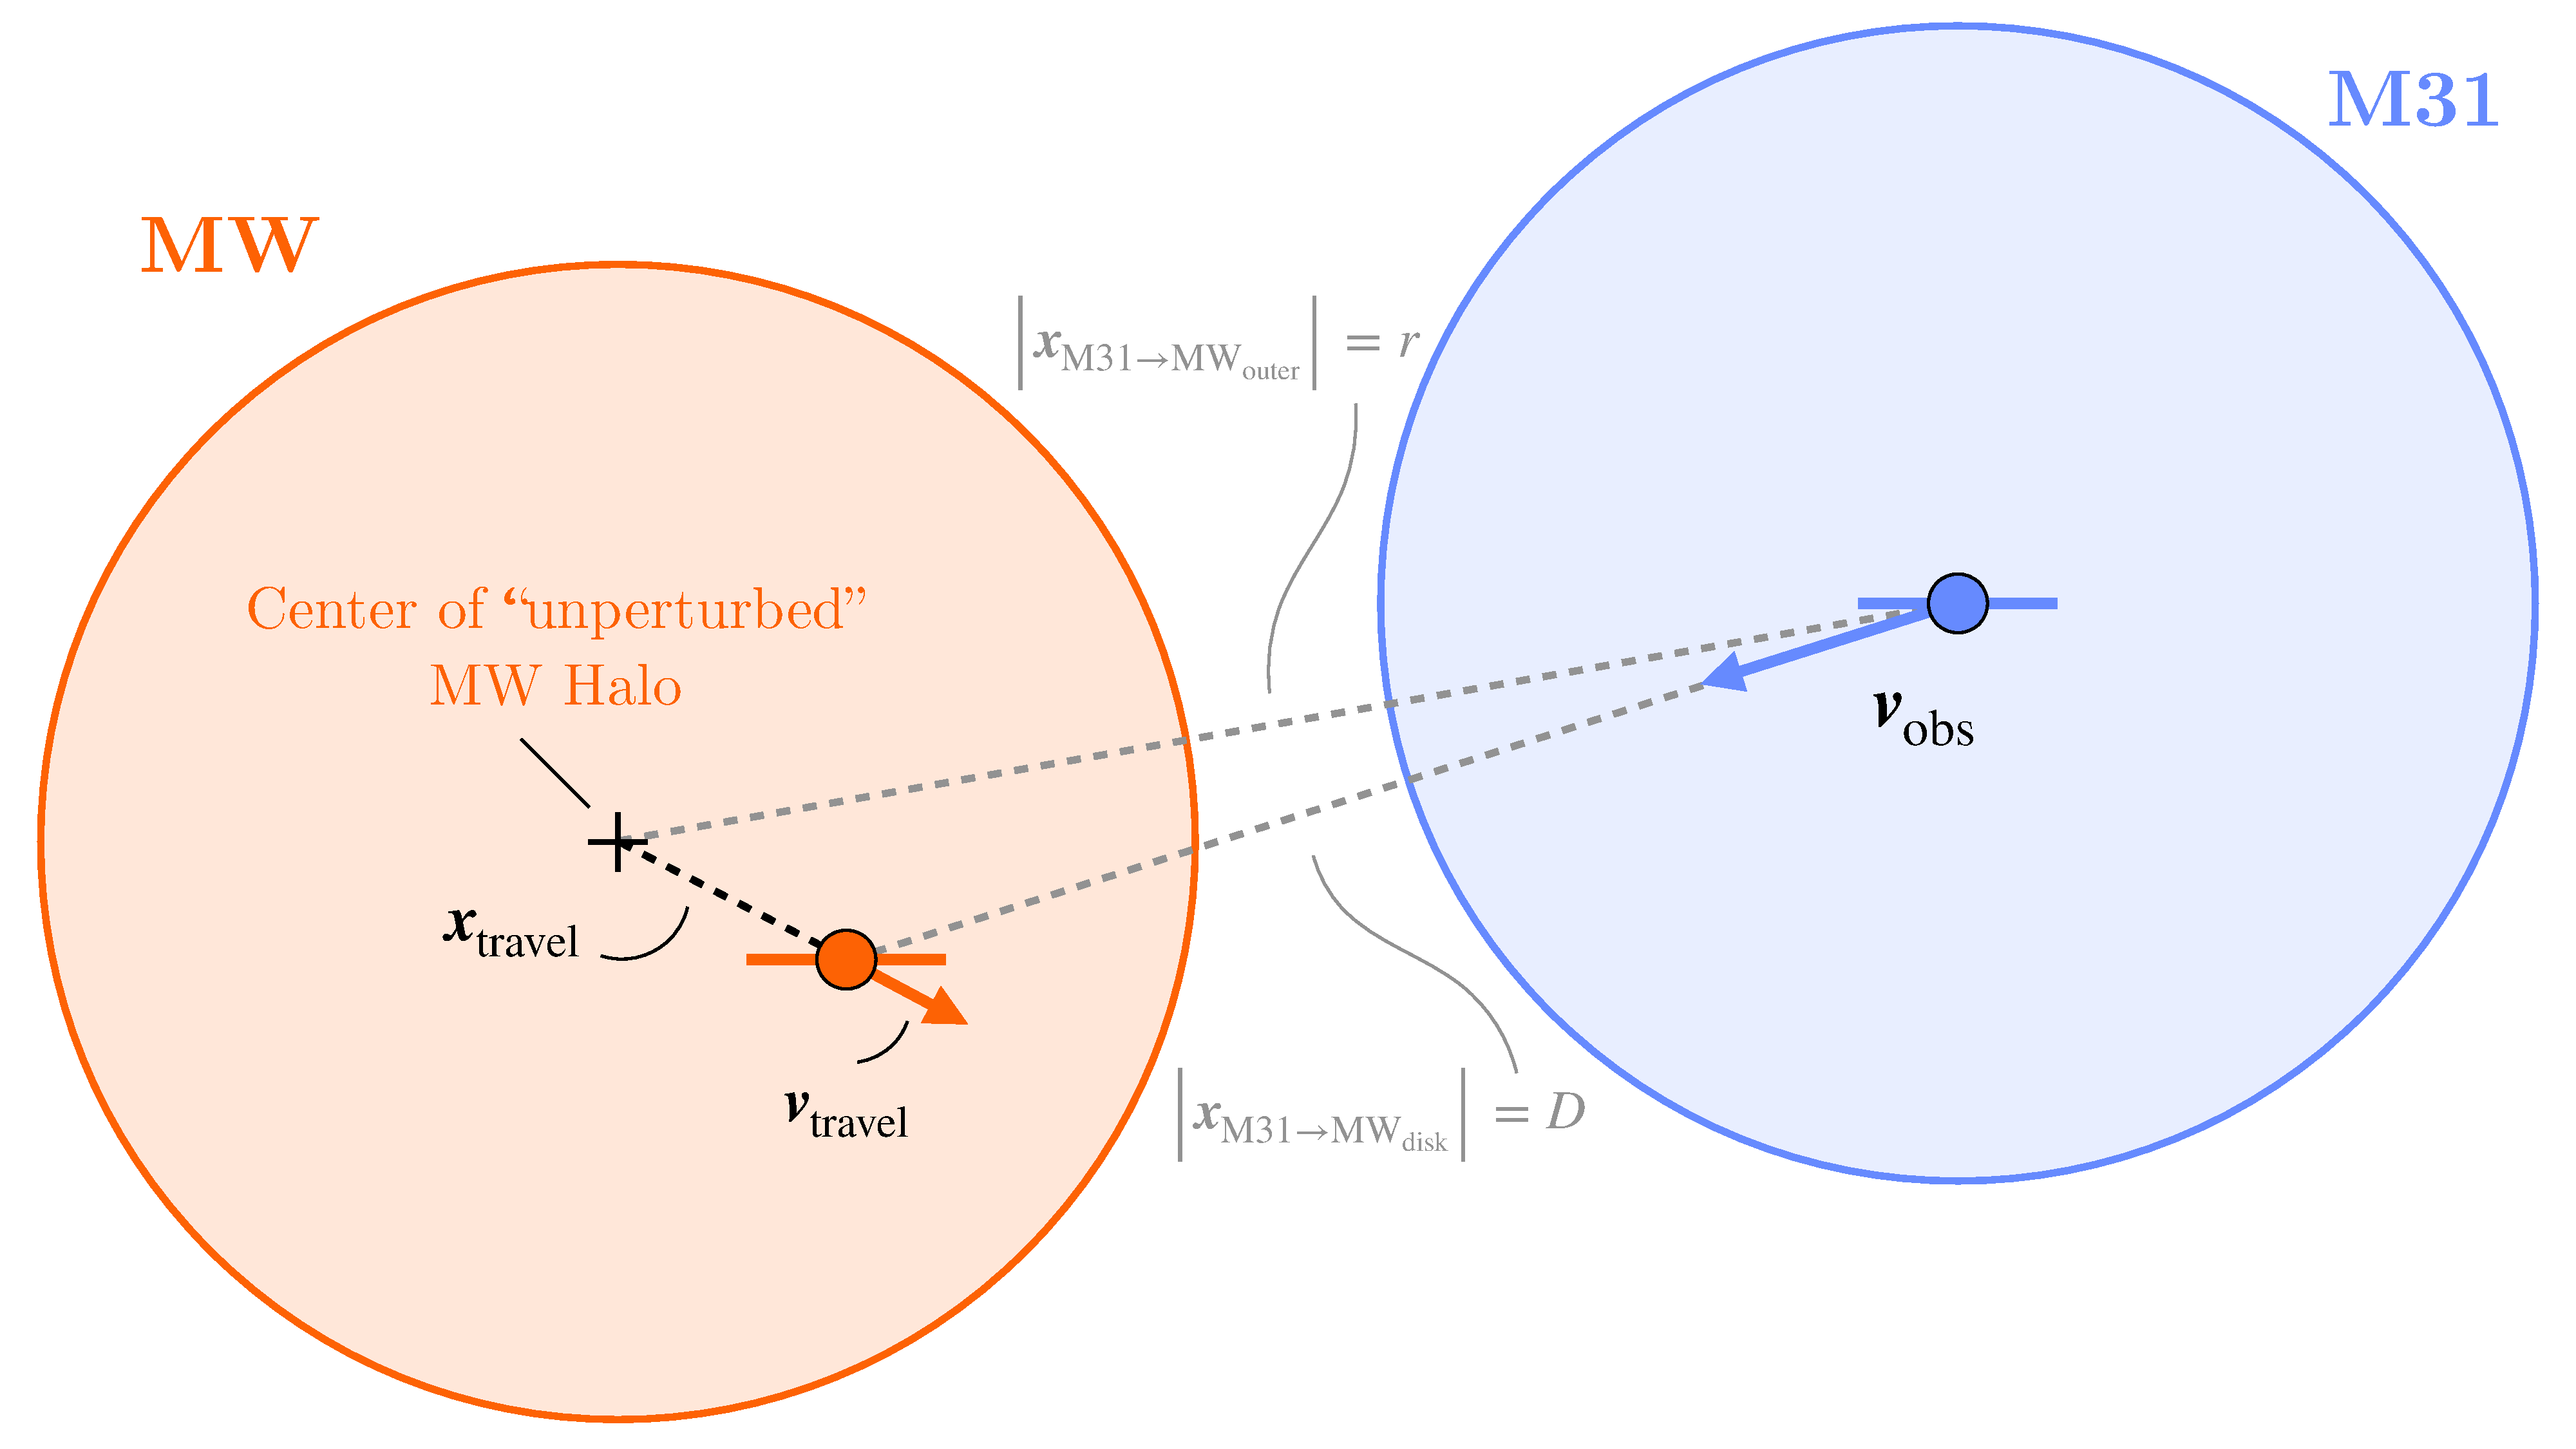
\includegraphics[width=0.8\textwidth]{schematic.pdf}
  \caption{
    Schematic of the MW and M31 system, not to scale. The shaded regions
    represent the halos of both galaxies. Shown are an artistic representation
    of the velocity and position vectors that are relevant in our model,
    including:
    $D=\pos{M31}{\odot}$, the measured distance to M31;
    $\pos{M31}{\mwouter}$, the distance between the centers of both halos;
    and $\boldsymbol{v}_{\rm obs}$, the measured 3D velocity of M31.
    Finally, \xtrav\ and \vtrav\ are the present distance and velocity
    between the center of the MW halo and the center of the MW disk.
    For this study, we assume $\xtrav\ll r,D$, and $\vtrav = 32\pm4 \kms$
    from~\cite{Petersen2021}.
    }
  \label{fig:schematic}
\end{figure*}


%%%%%%%%%%%%%%%%%%%%%%%%%%%%%%%%%%%
\subsection{Datasets}
\label{sec:datasets}
%%%%%%%%%%%%%%%%%%%%%%%%%%%%%%%%%%%
The present distance and relative velocity of M31, as well as the age of the
universe (used in Equation~\ref{eq:t}), are key observables that are used to
constrain our Timing Argument model. In this paper, we consider three different compilations of data to understand how different measurements might affect the
Timing Argument model with the addition of the travel velocity. In particular,
we consider two different M31 distance measures: an approximated distance
measure from~\cite{vdm2008}, and a more accurate Cepheid-based distance measure
from~\cite{Li2021}. We also consider two different M31 proper motion
measurements: \hst-based proper motions from~\cite{vdm2012}, and a more recent
\gaia\ eDR3-based proper motion measure from~\cite{Salomon2021}.

We have split these measurements into three compiled datasets:
\begin{description}
  %
  \item[vdMG08 Dist. + HST PM] the
  M31 distance measure from~\cite{vdm2008} and \hst\ proper motions
  from~\citet{vdm2012} -- the same dataset as used to constrain the Local Group
  mass via the Timing Argument
  in~\citet{vdm2012}
  %
  \item[Cepheid Dist. + Gaia PM]  a
  compilation of more recent M31 kinematic measurements, including a more
  precise Cepheid-based distance measure to M31 \citep{Li2021} and updated
  \gaia\ eDR3 proper motions from \citep{Salomon2021}.
  %
  \item[Cepheid Dist. + HST PM] a hybrid dataset with the Cepheid-based distance
  measure to M31 and the \hst-based proper motion measurement
  \citep{Li2021,vdm2012}.
\end{description}
The \hst-based proper motions were originally presented in~\cite{Sohn:2012},
and were then corrected for the internal kinematics and space motion of
M31 in~\cite{vdm2012},
from which we used the ``Weighted Average'' heliocentric
velocities in Table~3.\footnote{
Note that the referenced papers actually report velocity components and
uncertainties: To transform from velocity back to proper motions, we divide out
the adopted distance and deconvolve the distance uncertainty to obtain proper
motions and uncertainties of $\mu_{\alpha^*} = XX pm YY~\masyr$ and
$\mu_{\delta} = XX pm YY~\masyr$.\todo{Fill in the numberz!}.
}
The \textit{Gaia}-based M31 proper motion measurement is slightly larger than
the \hst\ proper motion of M31, leading to an increased implied transverse
velocity that, a priori, should lead to a higher inferred Local Group mass
compared to the more radial orbit implied by the \hst\ proper motions.
See Table~\ref{table:data} for numerical values used in each of these datasets.


\begin{table*}
  \begin{tabular}{lc|c|c}
    \hline\hline
      & \textbf{vdMG08 Dist. + HST PM} & \textbf{Cepheid Dist. + Gaia PM} & \textbf{Cepheid Dist. + HST PM}\\\hline
  $D~[\kpc]$ & $770 \pm 40\reflabel{a}$ &   $761\pm11~\kpc\reflabel{f}$  & $761\pm11\reflabel{f}$\\
  $v_{\rm rad}~[\kms]$ & $-301 \pm 1\reflabel{b}$ & $-301\pm 1\reflabel{b}$ & $-301\pm 1\reflabel{b}$ \\
  $\mu_{\alpha^*}~[\muasyr]$    & $34.30\pm 8.25\reflabel{c}$  & $48.98\pm 10.47\reflabel{g}$ & $34.30\pm 8.25\reflabel{c}$ \\
  $\mu_\delta~[\muasyr]$ & $-20.22 \pm 7.71$\reflabel{c} & $-36.85\pm 8.03\reflabel{g}$ & $-20.22 \pm 7.71$\reflabel{c} \\
  $\bs{v}_\odot$~[\kms]& $(11.1, 251.54, 7.25)\reflabel{d}$ & $(12.9, 245.6, 7.78)\reflabel{h}$ & $(12.9, 245.6, 7.78)$ \reflabel{h}\\
  $t_{\rm peri}~[\Gyr]$ & $13.75\pm 0.11\reflabel{e}$  & $13.801 \pm 0.024$ \reflabel{i} & $13.801 \pm 0.024$ \reflabel{i}\\
  \hline\hline
  \end{tabular}
  \tablerefs{$a.$ \cite{vdm2008},
   $b.$ \cite{Courteau1999},
   $c.$ \cite{vdm2012},\\
   $d.$ \cite{Schonrich2010,McMillan2011},
   $e.$ \cite{Jarosik2011},
   $f.$ \cite{Li2021},
   $g.$ \cite{Salomon2021},\\
   $h.$ \cite{Drimmel2018},
   $i.$ \cite{Planck2018}}
  % \tablenotetext{a}{\cite{vdm2008}}
  % \tablenotetext{b}{\cite{Li2021}}
  \caption{\label{table:data}
  Observational datasets used for comparison throughout analysis and their
  references. Each value is measured for M31 with
  respect to the sun. $D$ is the distance, $v_{\rm rad}$ is the radial velocity,
  $(\mu^*_{\alpha}, \mu_{\delta})$ are proper motions in RA cosdec and Dec, and
  (U$_{\rm pec}$, V$_{\rm pec}$+V$_0$, W$_{\rm pec}$) the solar motion with
  respect to the Galactic center. $t_{\rm peri}$ is the time elapsed since the
  last pericenter of the M31 Keplerian orbit, which in this case is the age of
  the Universe.
  }
\end{table*}


%%%%%%%%%%%%%%%%%%%%%%%%%%%%%%%%%%%%
\subsection{Bayesian Inference}
\label{sec:bayes}
%%%%%%%%%%%%%%%%%%%%%%%%%%%%%%%%%%%%

We construct a likelihood function for the observed heliocentric distance,
proper motion components, and radial velocity of M31, along with the time since
last pericenter, given the four parameters of the Timing Argument model $(\mlg,
a, e, \eta)$.
We then adopt prior probability distribution functions (pdfs) for the parameters
and use these pdfs to compute the posterior pdf over the parameters given the
data in order to generate samples from the posterior pdf using a Markov Chain
Monte Carlo (MCMC) method.

In detail, we first use the four Timing Argument parameters to compute the
present-day separation between the MW and M31 halos and their relative radial and
tangential velocities as defined in Equations~\ref{eq:r}--\ref{eq:vtan}.
These velocity components represent the relative velocity M31 would have as
observed from the center of an unperturbed MW halo.
We then use the measured ``travel velocity'' of the MW disk,
\vtrav, to find the relative velocity of M31 with respect to the center of the moving MW disk (i.e. a moving MW Galactocentric frame).
We finally transform from this Galactocentric frame to a heliocentric
reference frame moving with the solar system barycenter (i.e. ICRS coordinates).
At this final stage, we must introduce an additional nuisance parameter $\alpha$
that represents the orientation of the MW--M31 orbital plane as it intersects
the tangent plane located at the sky position of M31 as viewed from the MW disk
center --- this parameter is needed to convert from the two-dimensional velocity
components given by Equations~\ref{eq:vrad}--\ref{eq:vtan} to the
three-dimensional velocity components represented by the two proper motion
components and the radial velocity of M31.
% This is necessary because the Kepler equations only provide the magnitude of the
% tangential velocity (i.e. Equation~\ref{eq:vtan}), but in order to compute
% proper motion components we must also know the exact orientation of the M31
% velocity vector.
However, we stress that this position angle has no impact on the fundamental
dynamical parameters and is only used for coordinate transformations.

We specify this model using the \texttt{Python} probabilistic programming
package \texttt{pymc3}~\citep{Salvatier2016} and use the No-U-Turn Sampler
(NUTS) \citep{Homan2014} implemented in \texttt{pymc3} to generate samples from
this posterior pdf, given data from each of the datasets defined in
Table~\ref{table:data}.
We sample over the parameters Local Group mass $\mlg$, the present-day MW--M31
halo separation $r$, log eccentricity $\ln\left(1 - e\right)$, eccentric anomaly
$\eta$, and the orbital plane orientation nuisance parameter $\alpha$.
Our adopted prior pdfs are defined in Table~\ref{table:priors}.
% We set the priors as follows:
% \kc{do we need the following bullets if we have the table?}
% \begin{itemize}
%   \item Mass of the Local Group $\mlg$: we use a broad, truncated normal
%   distribution centered on a past measured value of the local group mass.
%   \item Present MW--M31 separation $r$: we again use a broad, truncated normal
%   distribution centered on past measurements of the distance to M31.
%   \item Eccentricity $e$: we assume a uniform prior on eccentricity but sample
%   in the transformed parameter $\ln(1-e)$ to improve the acceptance fraction
%   when generating posterior samples.
%   \item Eccentric anomaly $\eta$: we assume a uniform prior.
%   \item Orbital plane orientation $\alpha$: we assume a uniform prior.
% \end{itemize}
% This information is summarized in Table~\ref{table:priors}.
For each dataset, we run the sampler with 4 chains for 4,000 tuning steps and
40,000 draws.

% \begin{equation}
%   \mathcal{L}(| \boldsymbol{S})
% \end{equation}
% where $\boldsymbol{S} = ($\mlg$, a, e, \eta)$

% TODO: Letters have a 1 table max limit, so we might have to move the prior
% details into the list above. But we could always submit as a short regular
% paper instead of a letter...
\begin{table}
  \centering
  \begin{tabular}{lc}
  \hline\hline
  Prior  & Description \\\hline
  \mlg: $\mathcal{N}_T(4.5,3)\times10^{12}\Msun$ & Mass of the Local Group\\
  %
  $r$: $\mathcal{N}_T(700,100)$kpc & Distance from M31 to $\mwdisk$\\
  %
  $\ln(1-e)$: $\mathcal{U}(-10,0)$ & Eccentricity (close to 1) \\
  %
  $\eta$: $\mathcal{U}(-\pi, \pi)$ & Eccentric anomaly\\
  \multirow{2}{*}{$\alpha$: $\mathcal{U}(-\pi, \pi)$} & Position angle of M31 orbital\\
  & plane from MW disk center\\
  \hline\hline
  \end{tabular}
  \caption{\label{table:priors} A description of our adopted prior probability
  distribution functions over the Timing Argument model parameters.
  Here, $\mathcal{U}(a, b)$ represents a uniform distribution over the domain
  $(a, b)$, and $\mathcal{N}_T(\mu, \sigma)$ represents a truncated Normal
  distribution with mean $\mu$ and standard-deviation $\sigma$.
  We truncate the mass prior pdf to the range $(0.5, 20)\times10^{12} \Msun$ and
  the radius prior pdf to the range $(100, 10^{4})\,\kpc$.
  }
\end{table}


%%%%%%%%%%%%%%%%%%%%%%%%%%%%%%%%%%%
\section{Results: Local group mass estimates}
%%%%%%%%%%%%%%%%%%%%%%%%%%%%%%%%%%%
\label{sec:results}
% \kc{Include the velocity vector of M31 from the halo frame?}

\begin{figure*}[htb]
  \centering
  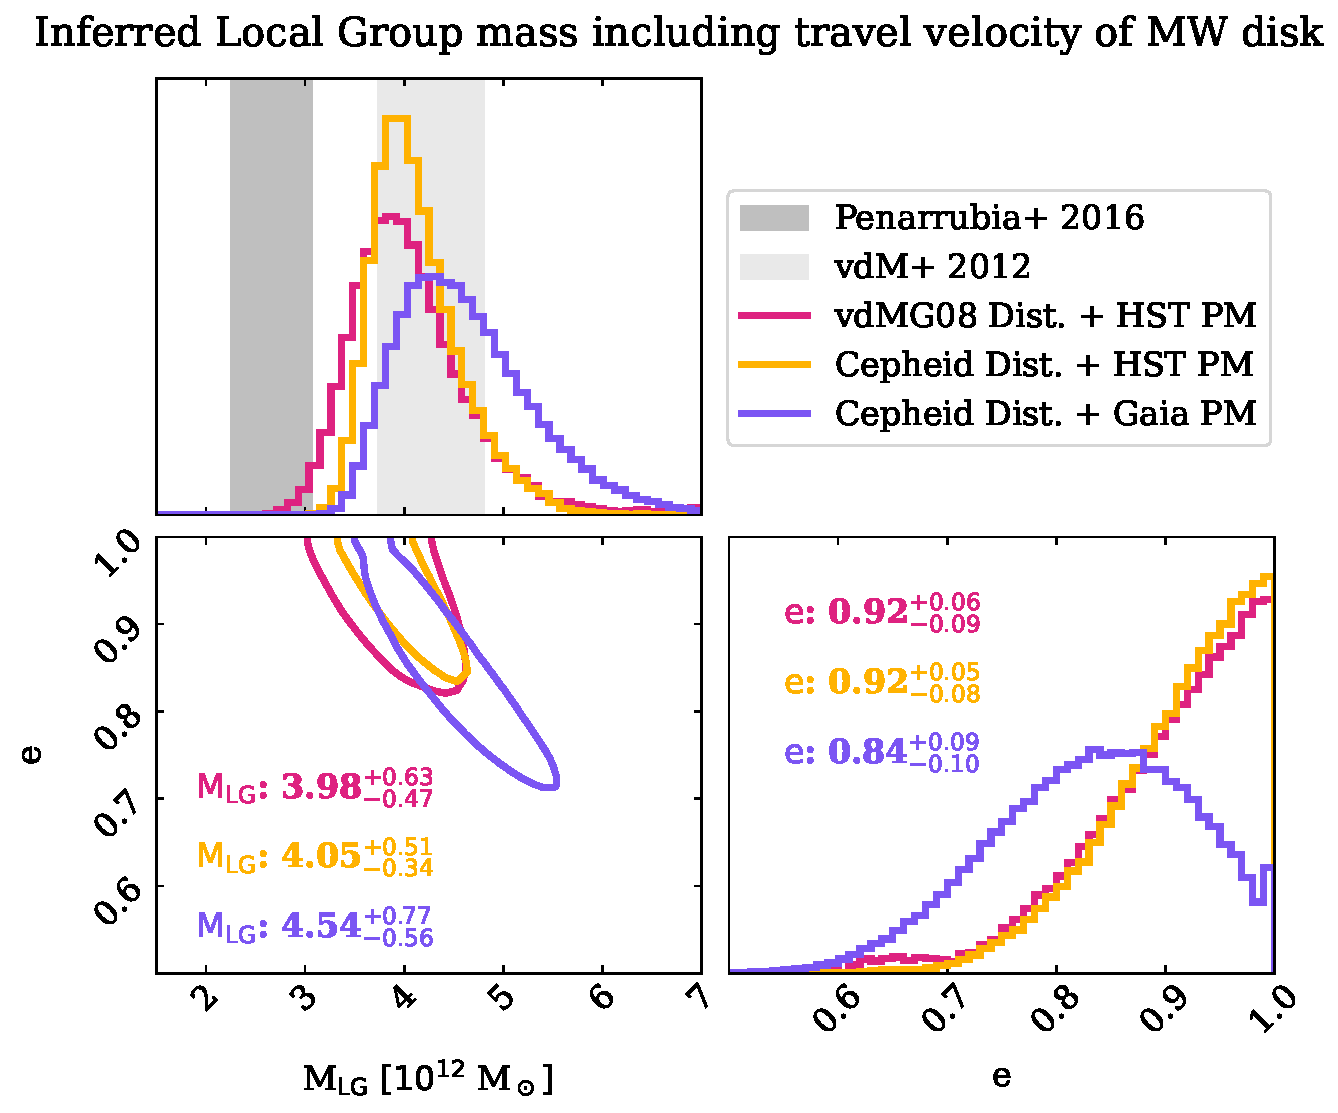
\includegraphics[width=0.8\textwidth,trim = 2.3cm 1.5cm 1cm 0cm,clip=true]
  {analyze-runs-contour.pdf}
  \caption{\label{fig:contour} 68\% credible regions of sampled posterior
  distributions with three observational datasets for a subset of our model
  parameters: the total mass of the Local Group (\mlg)
  and the eccentricity of the orbit of M31 about a fixed MW ($e$).
  Masses (in units of $10^{12}\Msun$) reported in the bottom left panel are
  the median mass and 68\% credible region for each dataset.
  The shaded regions in the upper left panel are the 68\% credible region mass
  estimates of previous TA studies from~\cite{vdm2012}
  and~\cite{Penarrubia2016}.
   %
  The more radial orbit implied by the~\cite{vdm2012} \textit{HST} proper
  motions leads to a lower inferred \mlg\ and a higher
  eccentricity, while the larger \textit{Gaia} proper motions of
  ~\cite{Salomon2021} yield a more circular orbit, and thus a lower eccentricity
   and higher mass system.
   }
\end{figure*}

% We use recent measurements of the present-day kinematics of M31 as observed from the solar system, updated measurements of the solar position and motion with respect to the Milky Way center, and a recent measurement of the velocity of the Milky Way disk with respect to the outer stellar halo to measure the mass of the Local Group using observed kinematics of M31.

We use a Bayesian implementation of a Timing Argument model to infer the mass of
the Local Group and the distance between M31 and the Milky Way.
Our model of the Local Group accounts for the observed travel velocity of
the Milky Way disk from~\cite{Petersen2021}, and results in new,
less-biased constraints on the mass of the Local Group.

We find that our model prefers lower Local Group masses and a lower eccentricity
orbit compared to models that do not include the travel velocity of the MW disk.
We also find that the inferred mass is larger and the LG orbit is less eccentric
when using the (larger) \gaia\ proper motion of M31.
Figure~\ref{fig:contour} is a summary of our key results, showing the 68\%
credible regions from the sampled posterior pdfs of the LG mass \mlg\ and
eccentricity $e$ (lower left panel).
The upper left panel shows the marginal posterior pdfs over LG mass for each of
the datasets (histogram curves) and with 68\% credible regions plotted for two
prior LG mass measurements (gray shaded bands).
To summarize: With dataset \textit{vdMG08 Dist. + HST PM}, we find a
median posterior LG mass of $\mlg = 3.98 ^{+0.63}_{-0.47}\times10^{12}~\Msun$
(where error
bars here report the 68\% credible regions around the median), which is
roughly $0.3\times 10^{12}~\Msun$ smaller than reported in \cite{vdm2012} for
the same dataset.
With the updated dataset containing \textit{Cepheid Dist + Gaia PM}, we find
$\mlg = 4.54 ^{+0.77}_{-0.56}\times10^{12}~\Msun$, while for the combined
 \textit{Cepheid Dist. + HST PM} dataset, we find
 $\mlg = 4.05^{+0.51}_{-0.34}\times 10^{12}~\Msun$.

For both datasets that use the HST proper motions of M31, we
find that the inferred orbital eccentricity is consistent with a radial orbit.
Using the \gaia-based proper motions \citep{Salomon2021} leads to a finite
inferred LG orbital eccentricity of $e\sim 0.85$ and therefore a larger inferred
LG mass.
However, enforcing $e=1$ (i.e. a radial LG orbit) produces very consistent mass
estimates between the datasets considered, implying a LG mass $\mlg = 3.6
\pm 0.3 \times 10^{12}~\Msun$.


\begin{figure}[htb]
    \centering
    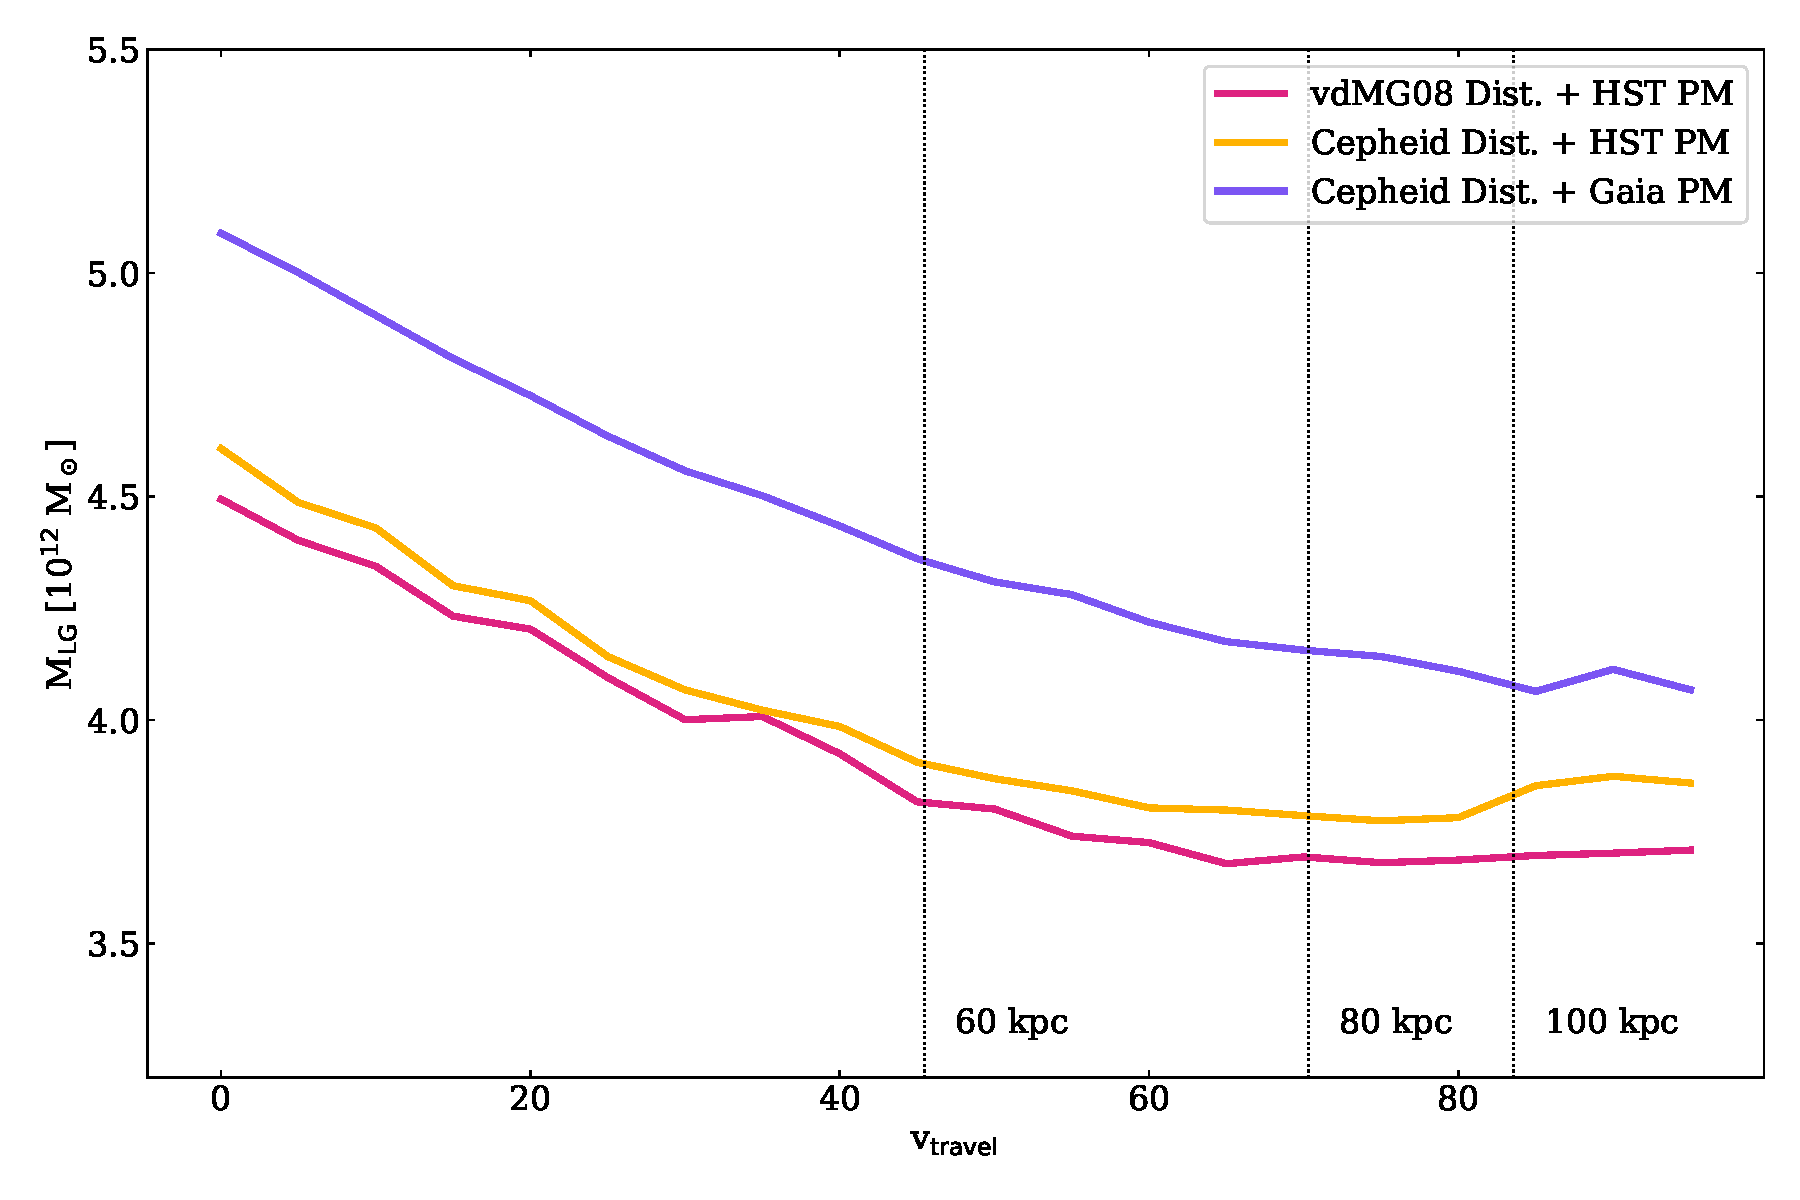
\includegraphics[width=\columnwidth]{analyze-runs-MvsV.pdf}
    \caption{\label{fig:mvsv}
    Mean inferred Local Group mass as a function of travel velocity
    magnitude of the MW disk.
    The larger \textit{Gaia} proper motions (purple) lead to higher transverse
    motion and thus higher mass than either of the \textit{HST} proper motion
    datasets (pink and yellow), though they display the same general trends with
     increasing travel velocity.
    The solid vertical line and accompanying shaded region represent the median
    and 67\% confidence interval of the travel velocity measured
    by~\cite{Petersen2021} of $\vtrav=32\pm 4\kms$.
    The dotted vertical lines represent simulated travel velocities for
    stellar tracers at different distances in~\cite{Garavito-Camargo2021b}.
    \textbf{The inclusion of the travel velocity of the MW disk systematically
    lowers the inferred mass of the Local Group} regardless of observational
    dataset.
    }
  \end{figure}

% APW SAYS: I think we can remove this figure and just discuss what it shows in
% the text.
% \begin{figure}[htb]
%     \centering
%     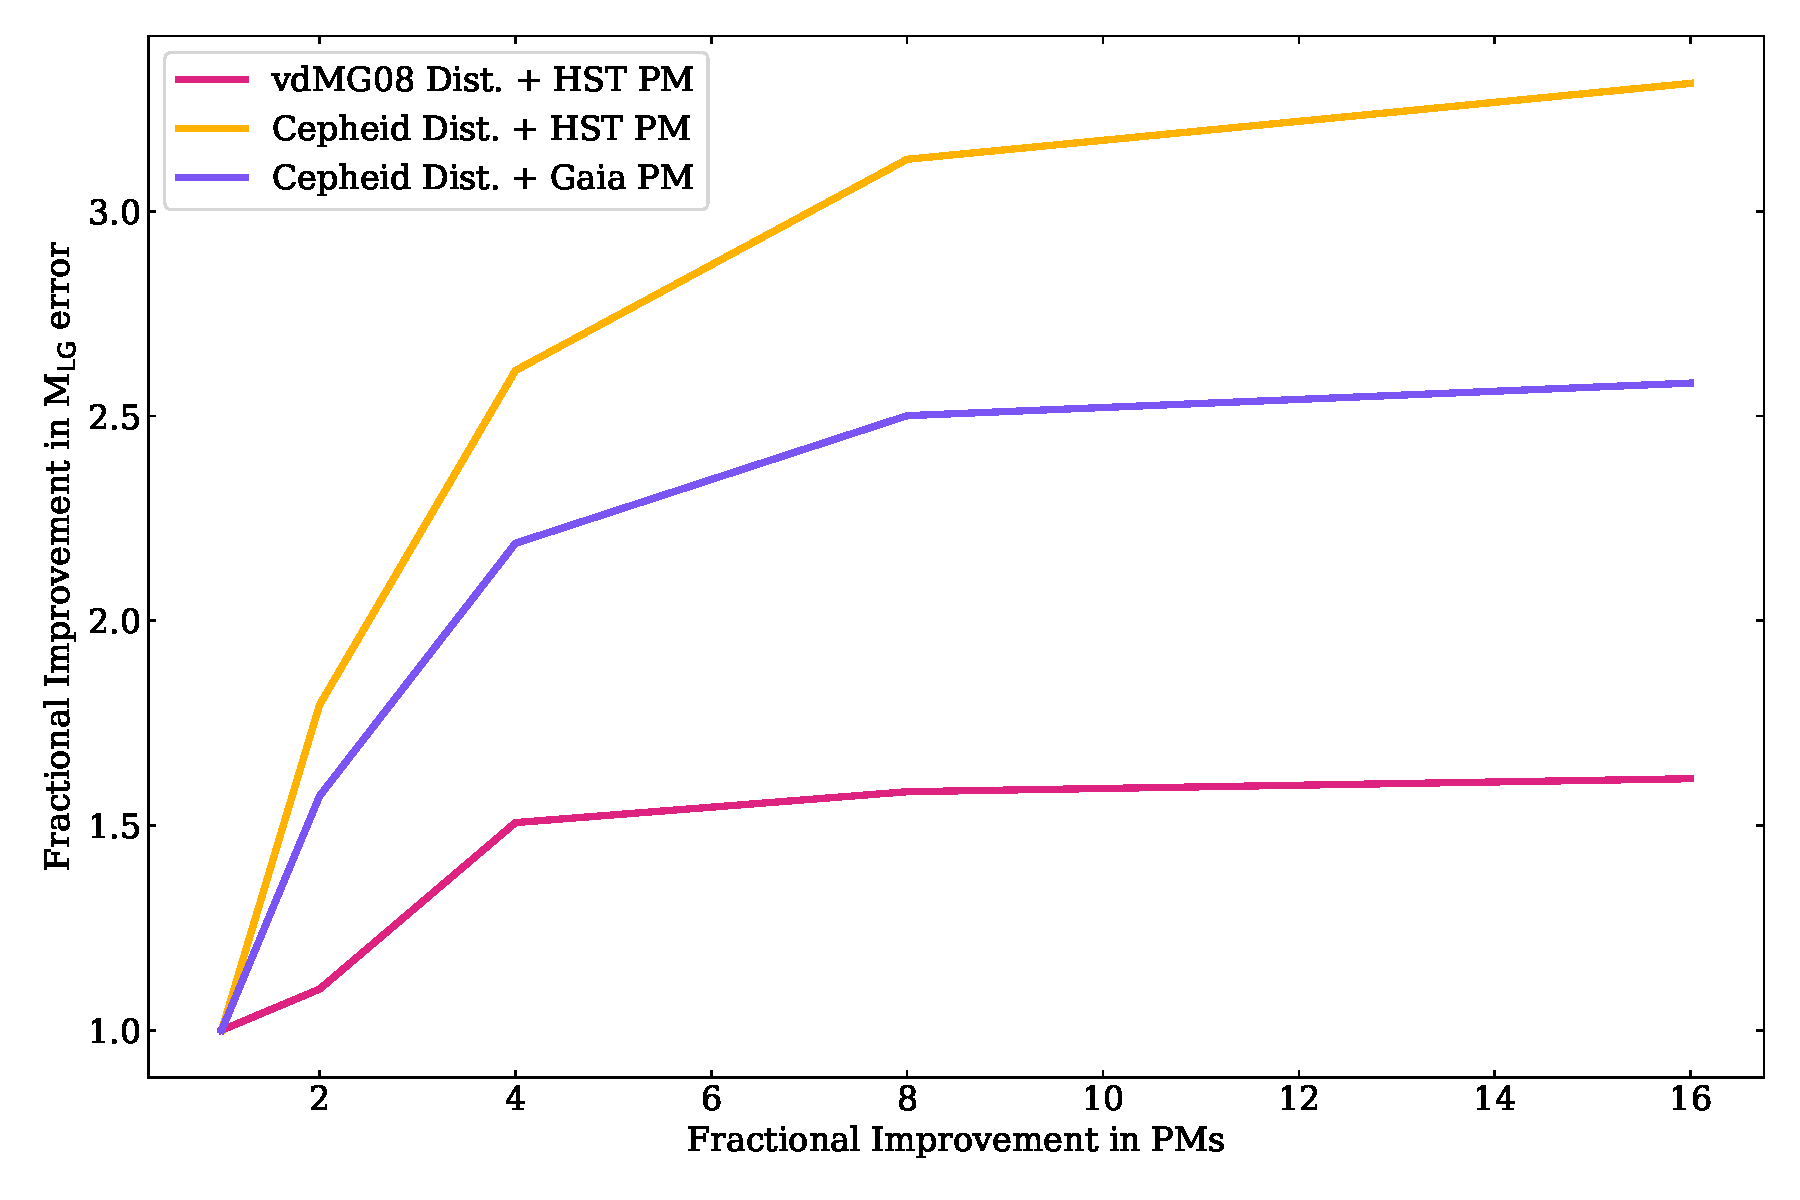
\includegraphics[width=\c\todo{
% \apw{Add a paragraph comparing our measurements to other values (e.g., summarize aspects of your Table 3)}}

% \todo{Suggested outline:}
% \todo{- There are two ways of measuring LG mass: go after it directly with LV dynamics / Timing Argument, or measure MW/M31 separately and add the masses}

% \todo{- Historically, LG dynamics-inferred masses are larger than adding MW+M31 masses: recap rough numbers from your Table 3 (LG dynamics masses have been upwards of $4\times 10^{12}$, adding independent mass measures closer to 2--2.5)}

% \todo{- One exception is the Penarrubia2016 method, ... (use sentences from paragraph below to describe)}

% \todo{- Our value is still larger than most added MW+M31 values (except Cosmo sims), but brings it closer to MW+M31}

% \todo{- Not surprising there is some discrepancy because MW/M31 total mass estimates do not measure full extent of DM distribution and have to extrapolate - there are large uncertainties}

% \todo{- Other TA models and what their differences have been. Namely, here compare Benisty and the fact that they use:
% model-dependent transverse velocity corrections
% Gaia PMs only}


% \todo{~\cite{Penarrubia2016} finds a Local Group mass of ($\sim2.64\pm0.4\times
% 10^{12}~\Msun$) which is significantly lower than our expectations, although this
% constraint combines the observed kinematics of 35 Local Volume galaxies in
% addition to the dynamics of the M31--MW system.
% Each of the Local Volume Galaxies is fit to a radial Keplerian orbital model.
% However, inclusion of any transverse motion will increase the inferred total
% mass of the system, so it is likely the assumption of radial orbits leads to
% an underestimate of the mass of the Local Group with LV galaxies only.
% Including the dynamics of the M31--MW system increased their recovered
% total mass by $0.6\times10^{12}~\Msun$. This is different from \citet{Penarrubia2016} who
% instead parametrize this term as a function of an additional parameter that sets
% the mass ratio of the LMC and the MW.}

% \todo{The \cite{Benisty2022} paper reports a Local Group TA mass of
% $5.6^{+1.6}_{-1.2}\times10^{12}\Msun$ after correcting for the reflex motion
% of the MW induced by the LMC, which is roughly 25\% larger than our findings.
% The discrepancy is likely due to differences in correcting for the reflex motion
% of the MW disk.
% They find that cosmic bias lowers the TA mass by an additional 40\%.
% The large errorbars are likely due to uncertainties in the orbital modelling of
% M31 about the combined MW--LMC system.}olumnwidth]{analyze-runs-deltaMvsPM.pdf}
%     \caption{\label{fig:mvspm} Improvement in the inferred Local Group mass as a function of fractional improvement in proper motion errors.
%     The standard deviation in the mass decreases with decreasing proper motion
%     error, and in particular, decrease by a factor of $\sim2.5$ for PMs that are
%     4 times smaller than in Dataset 2.
%     \textbf{As future \textit{Gaia} data releases provide improved proper motion errors, constraints on the Local Group mass from the Timing Argument can
%     improve by a factor of $>$2.}
%     }
% \end{figure}

%%%%%%%%%%%%%%%%%%%%%%%%%%%%%%%%%%%
\section{Discussion}
\label{sec:discussion}
%%%%%%%%%%%%%%%%%%%%%%%%%%%%%%%%%%%

\subsection{Comparing recent measurements of the Local Group mass}
There have been two primary pathways to measure the mass of the LG:
measure the masses of MW and M31 individually and add them, or go after the
total mass directly with LV dynamics, the Timing Argument, or cosmological
simulations.

Historically, total mass estimates are much larger than the sum of the
individual MW and M31 masses.
Typical LG masses are upwards of $4\times 10^{12}\Msun$, while the sum of
independent MW+M31 mass measures result in a total mass closer to
$2-2.5\times 10^{12}\Msun$, as can be seen in the collection of previous mass
estimates for the LG, M31, and the MW in Table~\ref{table:masses}.
It is not surprising that there is a discrepancy between the total and summed
values of the LG mass, since MW+M31 mass estimates do not measure the full
extent of the distribution of dark matter in the LG, and thus must extrapolate
in regions where there may be large uncertainties. \todo{citations?}


There have been a few exceptions in the trend of high total mass measurements,
namely in~\cite{Diaz2014} and~\cite{Penarrubia2016}.
\todo{describe the Diaz method}

Additionally, ~\cite{Penarrubia2016} finds a Local Group mass of
$\sim2.64\pm0.4\times 10^{12}~\Msun$, which is significantly lower than our
expectations, although this constraint combines the Timing Argument dynamics of
the M31--MW system in addition to the observed kinematics of 35 Local Volume
galaxies. They parametrize the offset of the LMC+MW barycenter from a
MW-only barycenter as a function of the mass ratio between the LMC and MW, and
find that the LMC likely has~$\sim25\%$ of the mass of the MW halo, resulting in
a large shift in the barycenter of the LMC+MW.
% Each of the Local Volume Galaxies is fit to a radial Keplerian orbital model.
% However, inclusion of any transverse motion will increase the inferred total
% mass of the system, so it is likely the assumption of radial orbits leads to
% an underestimate of the mass of the Local Group with LV galaxies only.
The recovered mass using only the dynamics of the LV galaxies was quite low
($\sim 2\times 10^{12}\Msun$),
including the Timing Argument dynamics of the MW--M31 system increased their
recovered total
mass by $0.6\times10^{12}~\Msun$.

Our LG mass estimates are consistent with a number of other recent studies that
estimate the mass of the LG through dynamical methods.
We find agreement with the previous Timing Argument model
of~\cite{vdm2012} which found a total mass
of $4.27\pm0.45\times 10^{12}\Msun$ (neglecting for cosmic bias and
scatter) using the same values for the distance and velocity of
M31 as in our \textit{vdMG08 Dist. + HST PM} dataset.

\cite{Zhai2020} found XXX.


Additionally, \cite{Benisty2022} recently used the Timing Argument to place constraints on the
LG mass while correcting for the reflex motion of the MW disk induced by the LMC. They find a LG mass of
$5.6^{+1.6}_{-1.2}\times10^{12}\Msun$, which is roughly 25\% larger than our findings, and that accounting for cosmic bias \& scatter lowers the mass by an additional 40\%.

The discrepancy between this study and the \cite{Benisty2022} work is likely due to differences in correcting for the motion of the MW disk. \cite{Benisty2022} estimated the contribution of the reflex motion of the MW disk to the observed values of the \todo{positions and} velocities


The large errorbars are likely due to uncertainties in the orbital modelling of
M31 about the combined MW--LMC system.
From intro ``Recent Timing Argument work by \cite{Benisty2022} modelled the orbital history
of M31 and the MW with and without a mass model of the LMC to estimate the
contribution of the reflex motion of the MW to the measured tangential and
radial velocities of M31, then applied these corrections to their model to
remove the impact of the LMC in their analysis.''
model-dependent transverse velocity corrections
Gaia PMs only




\subsection{Correction for ``Cosmic Bias''}

Given the simplicity of the Timing Argument dynamical model --- in particular,
the assumption that the MW and M31 are point masses with constant masses --- it
is reasonable to wonder whether this methodology provides unbiased estimates of
the true LG mass.
An early study of a dark-matter-only cosmological simulation found that the
Timing Argument applied to pairs of galaxies did provide unbiased estimates of
the sum of masses of the pairs \citep{LiWhite2008}.
However, more recently it was found that conditioning on LG-analogs with similar
radial and tangential velocities to the MW and M31 leads to slightly biased
(overestimated) inferred total masses of those systems \citep{Gonzalez2014,
Hartl2021}.
In this work, we do not attempt to ``correct'' our inferred LG masses for this
cosmic bias effect, because it is unclear whether cosmological simulations
accurately reproduce the detailed properties of LG systems.
Accounting for this effect would likely lower our LG mass measurements.


\subsection{Inclusion of \todo{Milky Way disk reflex motion in dynamics of the Local Group}}

As shown in our results above, including the \todo{reflex motion of the Milky Way disk
results in measurable differences in the estimated mass of the Local Group
through the Timing argument.
Ignoring this motion at its currently measured travel velocity}\footnote{Defined
as \todo{$\vel{\mwouter}{\mwdisk}$ above.} magnitude of $v_\textrm{travel} = 32~\kms$}
\citep{Petersen2021} leads to LG masses that are overestimated by $\sim30\%$.
However, the direction and magnitude of travel velocity is directly tied to the
inferred mass of the Local Group.
As it is currently measured, the (mean) direction of $\vel{\mwouter}{\mwdisk}$
is just $\sim$$60^\circ$ from the sky position of M31, meaning that the travel
velocity impacts the conversion of both M31's observed proper motion and radial
velocity from a Heliocentric reference frame to the ``outer halo'' reference
frame used above.
At fixed magnitude, if the true apex of the travel velocity motion is closer
(farther) to M31's sky position, it would primarily affect the radial velocity
(proper motions).

% Thus, the observed radial velocity of M31 will be higher than for an unperturbed MW halo. Since $-v_{rad}\propto M^{1/2}$ for an infalling system, a smaller (but still negative) radial velocity will yield a lower Local Group mass.

% The eccentricity decreases significantly for Dataset 2 compared to Dataset 1, due to the larger measured proper motions of Dataset 2.  Additionally, a smaller radial velocity corresponds to a lower eccentricity for a fixed mass and distance, which can be seen in the bottom right panel of~\ref{fig:contour}.

% bit about the stellar halo tracers and different distances etc
There is reason to believe that the recently measured MW disk travel velocity
could be a lower bound on the true value, which could be up to a factor of
$\sim$2--3 higher than the currently measured value.
Using an idealized simulation of an equilibrium dark matter halo that has a
recent merger with an LMC-like halo, \cite{Garavito-Camargo2021b} showed that
stellar halo tracers at different distances from the MW disk center may result
in different measured travel velocities.
\todo{while this simulation does not span previous mergers in the MW's history, it gives a good first order approximation of what we may expect}
% , and it is possible that the current measurement on $v_{travel}$ of 32km/s are just a lower bound on the actual reflex motion of the disk.
At fixed apex direction, a larger travel velocity would correspond to a lower
inferred LG mass.
Figure~\ref{fig:mvsv} shows the effect of increasing the measured travel
velocity magnitude and its impact on the inferred mass of the Local Group for
each of the datasets used in this work (see Section~\ref{sec:datasets}).
The vertical lines in this figure show the travel velocities that are predicted
for three tracer distances in simulations from~\cite{Garavito-Camargo2021b}
% \kc{why does the mass level off after 80kpc / 70km/s? }
Thus, future measurements of the travel velocity of the disk that use tracers at
larger distance around the MW stellar halo will likely lead to a lower inferred
Local Group mass.

\subsection{Improved \mlg\ constraints from future observations}

The biggest source of uncertainty in our empirically inferred LG mass $\mlg$ currently comes
from the proper motion measurements, which currently have signal-to-noise ratios
of just 3--4.
Future data releases from the \gaia\ Mission \citep{GaiaOverview2016} will lead
to more precise mean proper motions of M31 and thus more precise Timing Argument
constraints on the LG mass.
For example, between \gaia\ EDR3 and the end of the extended (10 year) mission,
the expected individual-source proper motion precision improvement for a $G=20$
source (i.e. an upper giant-branch star in M31) is a factor of $\sim$6.
Na\"ively scaling the proper motion uncertainties of M31 as measured with \gaia\
\citep{Salomon2021} by a factor of 6 leads to a $\sim2\times$ improvement in the
$\mlg$ precision.
Of course, the true improvement of the mean M31 proper motion with improved
individual source kinematics could be even better than linear because more
sources will be detected and usable in the measurement.


\subsection{The M31--M33 system\todo{change}}
\label{sec:discussion-m31}
\todo{short sentence about the M31 subsystem and how we absolutely do not attempt to add in a travel velocity.}
While M31 has a massive satellite (M33) of comparable mass ratio to the
MCs--Milky Way system, we do not expect there to be a significant reflex
velocity of M31's disk relative to its equivalent outer halo reference frame:
Recent work predicts that M33 is likely on first infall into the M31 halo and
has a much larger orbital pericenter than the MCs \citep[e.g.,][]{Patel2017a}.
On the other hand, M31 has likely experienced other significant mergers, as
evidenced by the double nucleus and Giant Southern Stream
\citep[e.g.][]{Ibata:2001, Font:2006}, but these were likely lower mass-ratio
mergers \citep[e.g.][]{Gilbert:2019, Milo:2022} and thus will have less of an
impact on the bulk motion of the M31 disk.
\todo{Given current knowledge of the M31 system and uncertainties in the orbital
histories of its most massive satellites, here we neglect the (likely
subdominant) reflex motion of the M31 disk.}
\todo{However, a measurement or upper limit on the M31 disk travel velocity would
enable further unbiased constraints on the Local Group mass.}

%%%%%%%%%%%%%%%%%%%%%%%%%%%%%%%%%%%
\section{Summary and Conclusions}
%%%%%%%%%%%%%%%%%%%%%%%%%%%%%%%%%%%
\label{sec:summary}
In this Letter, we use the Timing Argument to constrain the mass of the Local
Group by modeling the relative dynamics of the Milky Way (MW) and M31,
accounting for the recently-measured travel velocity of the MW disk with respect
to the outer stellar halo of the Galaxy.
We show that accounting for the travel velocity of the MW disk lowers the
inferred Local Group mass from the Timing Argument when compared to a prior
result using the same compilation of M31 kinematic measurements, finding $\mlg =
3.98\times 10^{12}~\Msun$.
Using more recent distance and proper motion measurements of M31 we find that
the orbit of the Local Group galaxies is less radial than previously found,
leading to a slightly higher inferred Local Group mass $\mlg = 4.54\times10^{12}~\Msun$.



\todo{clean up or rewrite a big-picture concluding paragraph?}
Our findings of a high mass Local Group are consistent with findings that the
mass of M31 is XXbig and the MW is $1-1.5\times10^{12}~\Msun$~\citep{??}.
However, this high group mass also has cosmological implications.
A high Local Group mass could also be consistent with tk that propose that M31
has undergone recent (XX Gyrs) major? accretion events with other massive
subhalos, resulting in morphological features like the Giant Southern Stream and
XX (what are other M31 things that indicate recent interactions? Do we think
much about M32? )

this allows us to take a purely empirical approach which differs from previous timing argument studies.

different velocity values of M31 to get different results for the same TA model setup.


what will improve the work in the future? proper motions etc. what could our work directly motivate?




it's critical to refine our measurements of PM of M31, as well as the measured travel velocity of the MW disk with tracers at further distance. it is crucial to clarify these measurements in the near future.


In this study, we account for the reflex motion of the MW disk
empirically, which allows us to avoid modelling uncertainties in the LMC orbital
history and mass profile, as well as uncertainties in the MW merger history.
Recent measurements of stellar tracers in the outer MW halo
by~\cite{Petersen2021} measure an instantaneous



% \subsection{Cosmological implications}
\begin{table*}
  \centering
  \begin{tabular}{clc|c}
    \hline\hline
    Mass & Method & Result ($ 10^{12}~\Msun$ ) & Citation \\\hline
    \multirow{9}{*}{\mlg}  &Timing & $3.6$ & \cite{Lynden-Bell:1981} \\
    &Timing (radial + cosmo sim calibration)  & $5.27$& \cite{LiWhite2008} \\
    &{Timing only} & {4.27$\pm$0.45} & \cite{vdm2012} \\
    &{Timing (3D + cosmic bias and scatter)} & {4.93$\pm$1.63} & \cite{vdm2012} \\
    & LG Dynamics &$2.5\pm0.4$ & \cite{Diaz2014}\\
    &{LV Galaxies + Timing Argument} & {2.64$\pm0.4$} & \cite{Penarrubia2016} \\
    & Cosmo Sims & 4.4$^{+2.4}_{-1.5}$ & \cite{Zhai2020}\\
    & TA + LMC & 5.6$^{+1.6}_{-1.2}$ & \cite{Benisty2022}\\
    & TA + CB + LMC & 3.4$^{+1.4}_{-1.1}$ & \cite{Benisty2022}\\

    %  &  &  \\
    \hline
    \multirow{4}{*}{\mmto}& Kinematics of M31 Sats & $1.4 \pm 0.4$ ($<$300 kpc) & \cite{Watkins2010}\\
    & LG Dynamics &$1.7\pm0.3$ & \cite{Diaz2014}\\
    & M31 Orbital Ang. Mom. & $1.37^{+1.39}_{-0.75}$ & \cite{Patel2017b}\\
    & Cosmo Sims & 2.5$^{+1.3}_{-1.1}$ & \cite{Zhai2020}\\

    \hline
    \multirow{5}{*}{\mmw}&  Kinematics of LG sats & $1.4 \pm 0.3$ ($<$300 kpc) & \cite{Watkins2010}\\

    & LG Dynamics &$0.8\pm0.5$ & \cite{Diaz2014}\\
    & MW Sats & $0.96^{+0.29}_{-0.28}$ & \cite{Patel2017b}\\
    & LMC Orbital Ang. Mom. & $1.02^{+0.77}_{-0.55}$ & \cite{Patel2017b}\\
    & Cosmo Sims & 1.5$^{+1.4}_{-0.7}$ & \cite{Zhai2020} \\
  \hline\hline
  \end{tabular}
  \caption{\label{table:masses}A collection of previous mass measurements from dynamics.}
\end{table*}

% Previous uses of the Timing Argument have placed constraints on the mass of the Local Group

% By including reflex motion, we move in the direction of the expected summed masses of the Milky Way and M31 which is good.

% How does the mass that we found compare to mass estimates from other means?
% - like hubble flow constraints, previous timing argument, previous MW--M31 measurements, etc.



% If our mass is higher, what does that mean?
% If our mass is lower, what does that mean?
% What does this high mass mean to the Local Group? What about to the
% constituents?

% What is context for mergers and M31 and why they might be
% related to the Local Group mass?


\begin{acknowledgements}

This project was started at the Big Apple Dynamics School (BADS) hosted by the
Flatiron Institute July--August 2021.
We greatly benefitted from discussions with the other students who attended the
BADS, and received helpful input from:
Kathryn Johnston (Columbia), Alex Riley (Texas A\&M)
\todo{Who else?}.
KC would like to thank Ekta Patel for sharing a collection of M31 mass measurements from the literature.
This work made use of the
\texttt{PyGaia}\footnote{https://github.com/agabrown/PyGaia} package: We
acknowledge the Gaia Project Scientist Support Team and the Gaia Data Processing
and Analysis Consortium (DPAC) for their work on this software tool.
This research made use of Astropy,\footnote{http://www.astropy.org} a
community-developed core Python package for Astronomy \citep{astropy:2013,
astropy:2018}.
\end{acknowledgements}

\software{
    Arviz \citep{arviz},
    Astropy \citep{astropy:2013, astropy:2018},
    gala \citep{gala},
    IPython \citep{ipython},
    matplotlib \citep{matplotlib},
    numpy \citep{numpy},
    pymc3 \citep{Salvatier2016},
    scipy \citep{scipy}
}

\appendix
Currently, appendix only includes the corner plots for all of the 5 model parameters for each of the three datasets.
\begin{figure*}[htb]
  \centering
  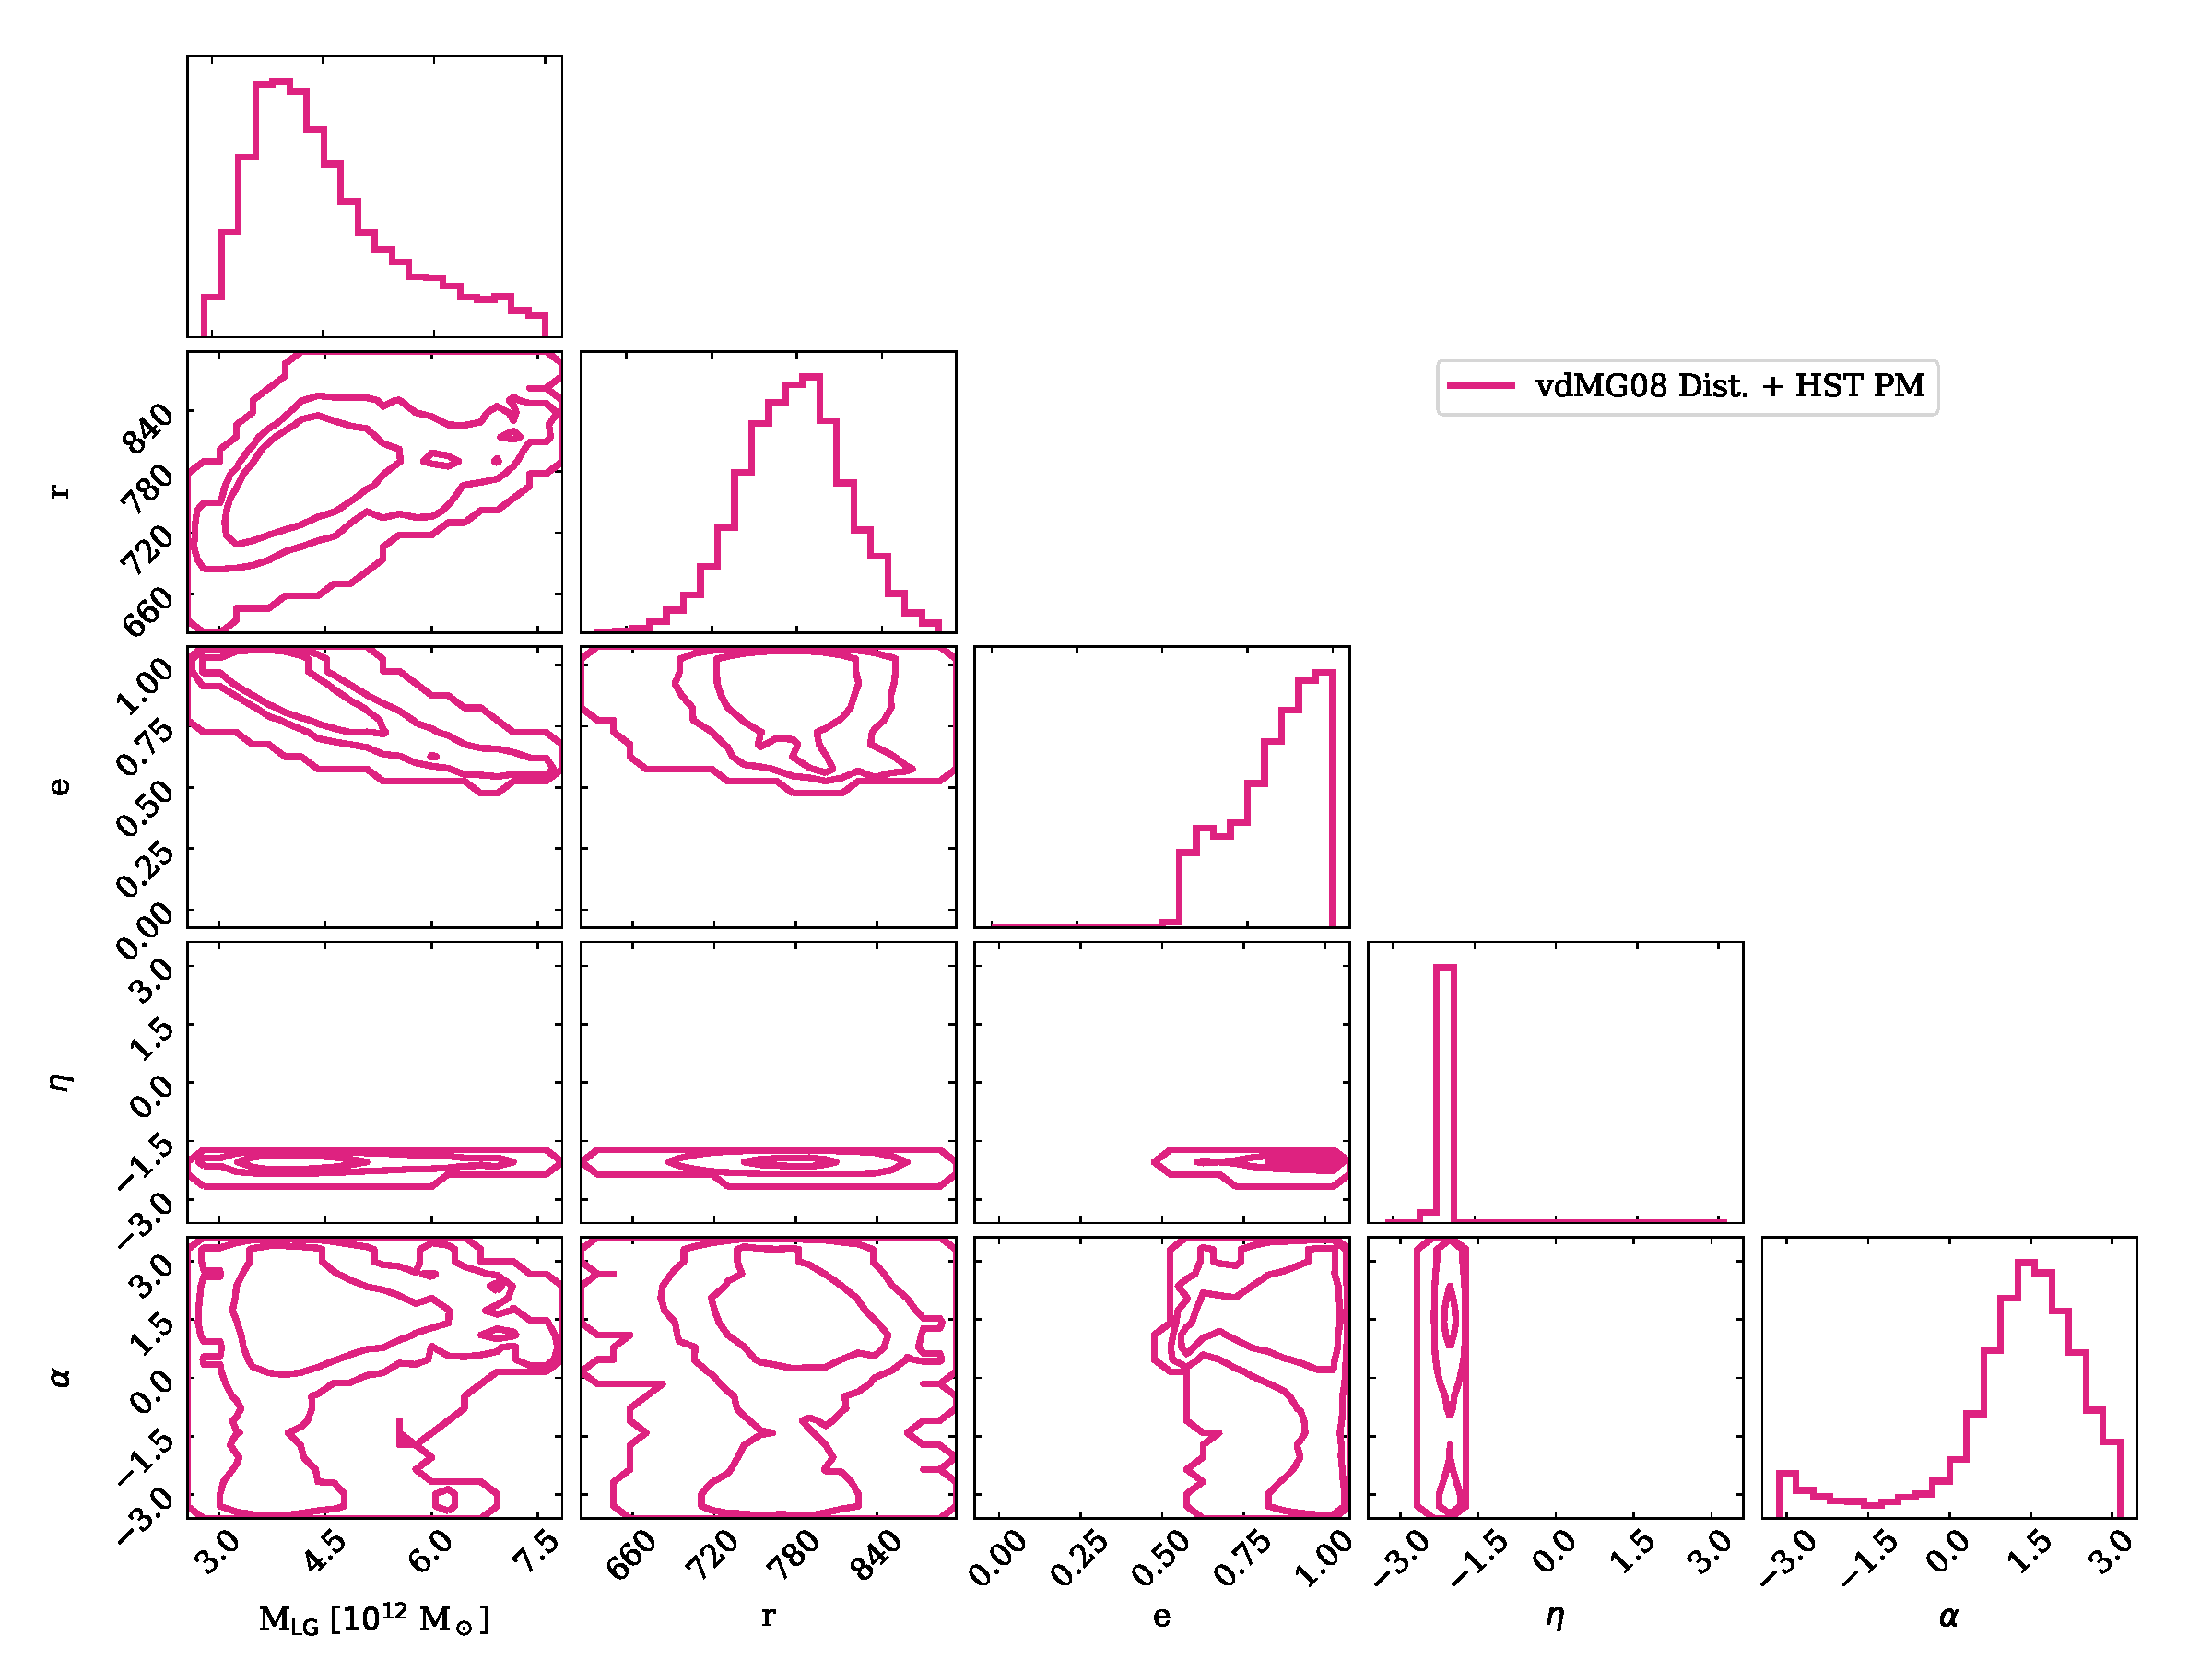
\includegraphics[width=0.8\columnwidth]{analyze-runs-all-vdm2012.pdf}
  \caption{\label{fig:contour-vdm}
  68\% and 95\% credible regions of sampled posterior distributions for all
  model parameters for the vdMG08 (how to make link to citation?) distance
  measurement $770\pm 40 \rm kpc$ and proper motions from \textit{HST}.
  }
\end{figure*}

\begin{figure}[htb]
  \centering
  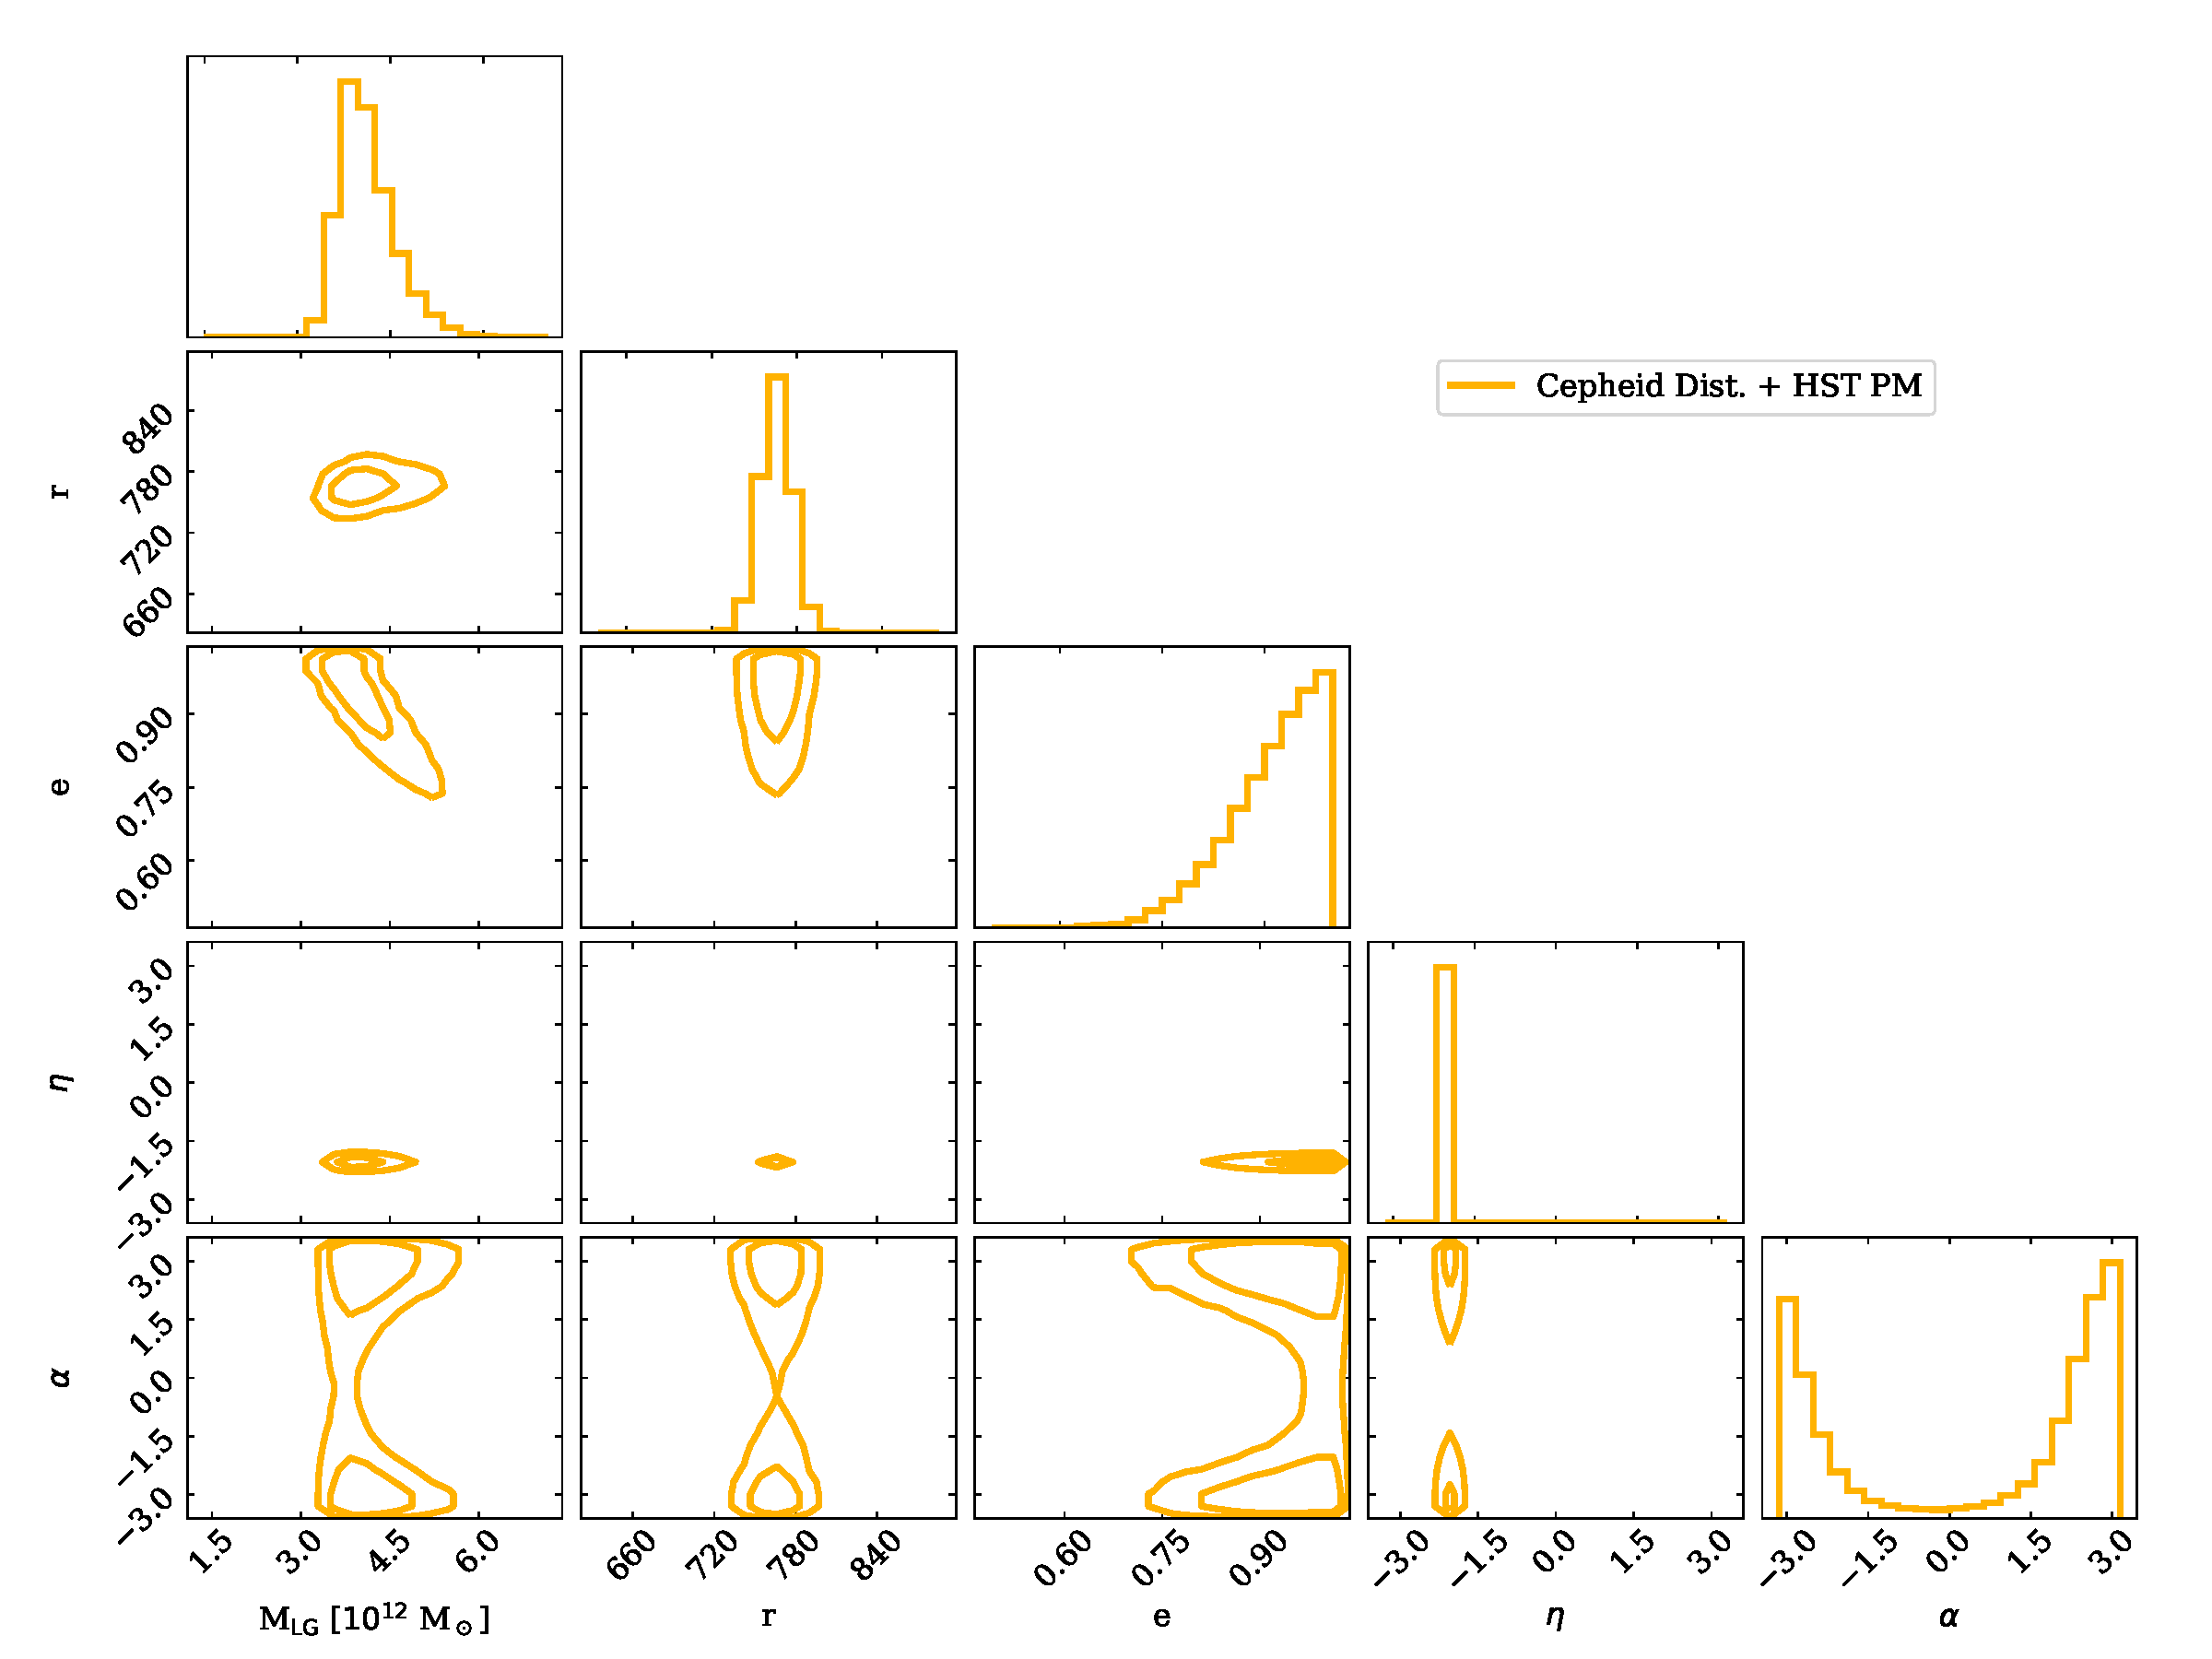
\includegraphics[width=0.8\columnwidth]{analyze-runs-all-Dataset3.pdf}
  \caption{\label{fig:contour-dataset3}
    68\% and 95\% credible regions of sampled posterior distributions for all
    model parameters for the vdMG08 (how to make link to citation?) distance
    measurement $770\rm kpc$ and proper motions from \textit{HST}.
  }
\end{figure}

\begin{figure*}[htb]
  \centering
  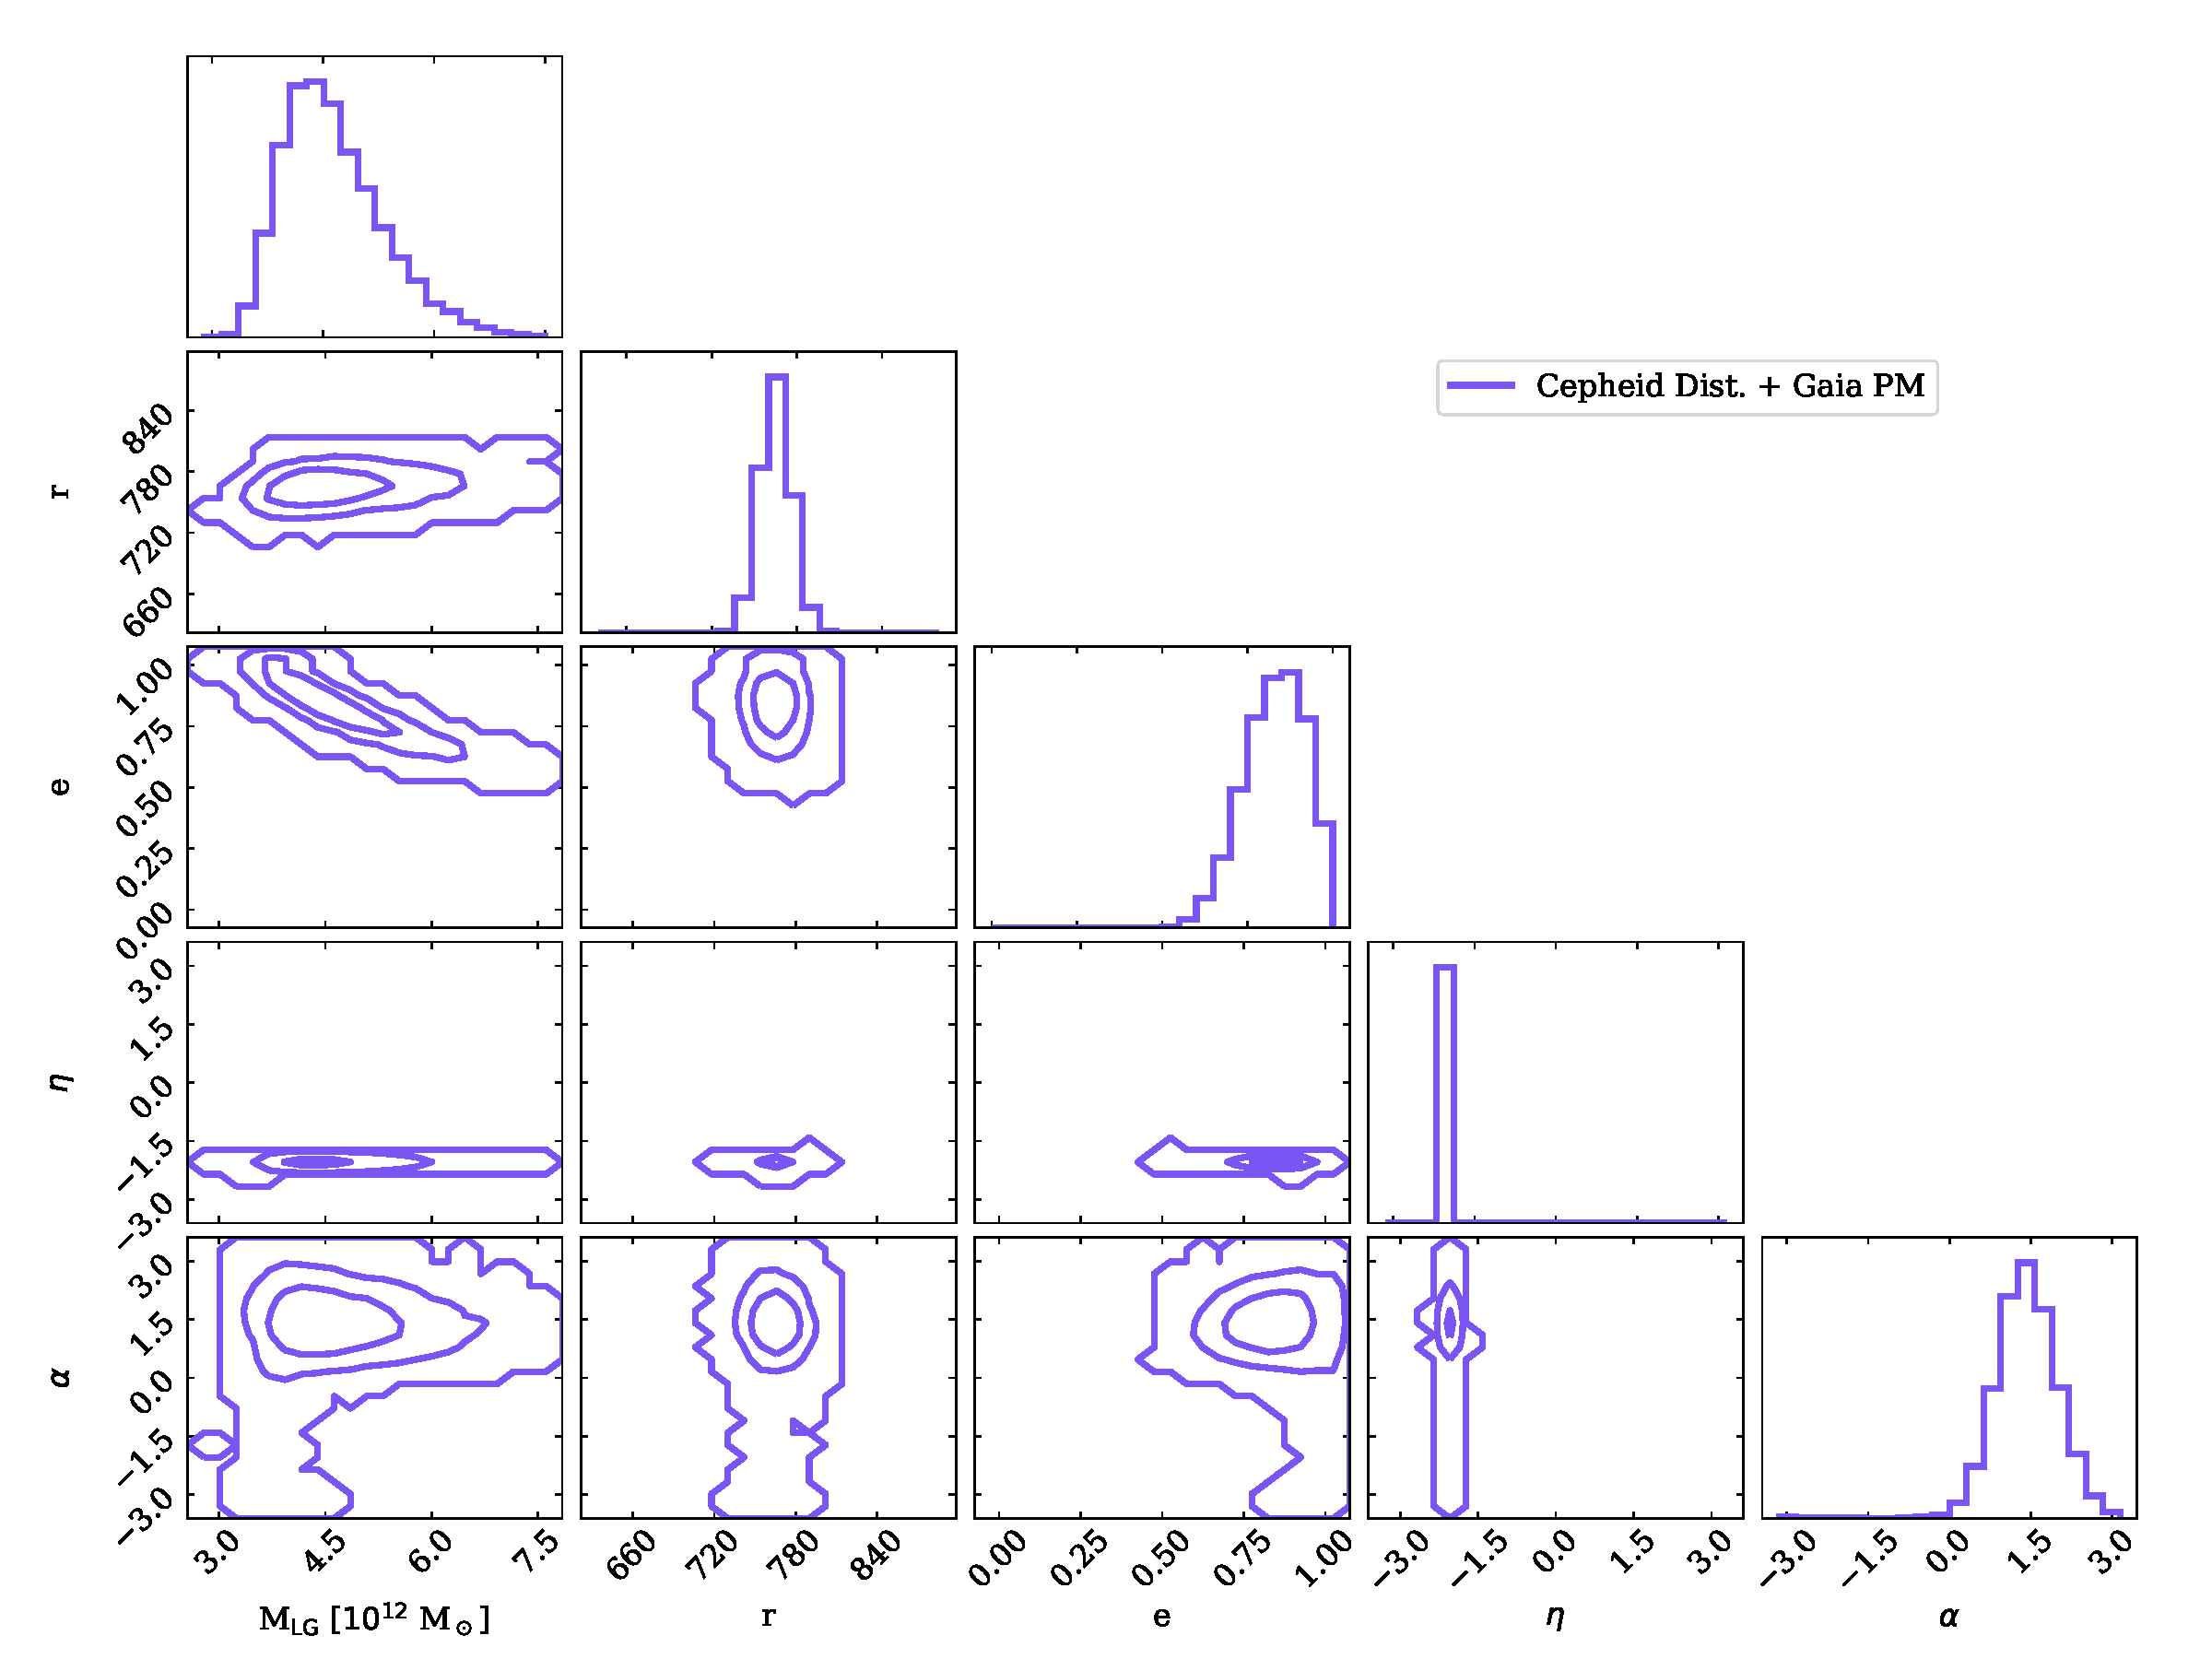
\includegraphics[width=0.8\columnwidth]{analyze-runs-all-fiducial2021.pdf}
  \caption{\label{fig:contour-fiducial}
  68\% and 95\% credible regions of sampled posterior distributions for all
  model parameters for the cepheid distance
  measurement $761\pm 11 \rm kpc$ and proper motions from \textit{Gaia}.
  }
\end{figure*}

\bibliography{refs}{}
\bibliographystyle{aasjournal}

\end{document}
